% NOW ADDED TO GIT

\documentclass [12pt,letterpaper]{report}

% Standard packages
\usepackage{amsmath}		% Extra math definitions
\usepackage{graphicx}		% PostScript figures
\usepackage{setspace}		% 1.5 spacing
\usepackage{longtable}          % Tables spanning pages
\usepackage{url}      % llt: nicely formatted URLs
\usepackage{booktabs}      % nice tables
\usepackage{float}
\restylefloat{table}
\restylefloat{figure}
\usepackage{caption}
\usepackage{subcaption}
\usepackage{hyperref}

\renewcommand{\floatpagefraction}{.8}	%if a float (figure, maybe table?) takes up more than 80% of a page, the page will only contain that float (default is 60%)

% subsubsubsection	BEGIN
\usepackage{titlesec}
\setcounter{secnumdepth}{4}
\titleformat{\paragraph}
{\normalfont\normalsize\bfseries}{\theparagraph}{1em}{}
\titlespacing*{\paragraph}
{0pt}{3.25ex plus 1ex minus .2ex}{1.5ex plus .2ex}
% subsubsubsection	END


% Custom packages
\usepackage[first]{datestamp}	% Datestamp on first page of each chapter
\usepackage[fancyhdr]{McECEThesis}	% Thesis style
\usepackage{McGillLogo}		% McGill University crest

% $Id: ThesisEx.tex,v 1.1 2005/06/09 12:48:46 kabal Exp $

\usepackage{color}
\def\headrulehook{\color{red}}		% Color the header rule

%===== page layout
% Define the side margins for a right-side page
\insidemargin = 1.3in
\outsidemargin = 0.8in

% Above margin is space above the header
% Below margin is space below footer
\abovemargin = 1.1in
\belowmargin = 0.75in


% PDF annotations (removed with 'final' option)
% An annotation alone adds a line; you can use % between the text and the annotation to avoid this.

\usepackage{xcolor}
\usepackage{pdfcomment}
% Here, specify your comment style (author name, color, icon, font, etc.)
\defineavatar{dan}{color=red,author={Danny}}
\defineavatar{jer}{color=blue,author={Jeremy}}
\defineavatar{ilja}{color=green,author={Ilja}}
% Some shortcuts producing annotations into the margin, with a vertical offset in option
\newcommand{\dan}[2][0pt]{\pdfcomment[avatar=dan,hoffset=#1,voffset=-6pt,opacity=.4]{#2}}
\newcommand{\jer}[2][0pt]{\pdfcomment[avatar=jer,hoffset=#1,voffset=6pt,opacity=.4]{#2}}
\newcommand{\ilja}[2][0pt]{\pdfcomment[avatar=ilja,hoffset=#1,voffset=-18pt,opacity=.4]{#2}}
% command to use \\ in pdfcomment to make a new line (otherwise use \textCR)
\pdfstringdefDisableCommands{\let\\\textCR}



%========= Document start

\begin {document}

%===== Title page

\title{%An Investigation of Low-Friction Surface Methods and the
Characterization and Application of a Variable-Friction Foot Device}
\author{Daniel Horodniczy}
\date{\Month\ \number\year}
\organization{%
  \\[0.2in]
  \McGillCrest {!}{1in}\\	% McGill University crest
  \\[0.1in]
  Department of Electrical \& Computer Engineering\\
  McGill University\\
  Montr\'{e}al, Qu\'{e}bec, Canada}
\note{%
  {\color{red} \hrule height 0.4ex}
  \vskip 2ex
  A thesis submitted to McGill University in partial fulfilment of the requirements for the degree of Master of Engineering.
  \vskip 2ex
  \copyright\ Daniel Horodniczy \the\year\ 
}

\maketitle

%===== Justification, spacing for the main text
\raggedbottom
\onehalfspacing
\pagenumbering{roman}

%===== Abstract, Sommaire & Acknowledgments
\section*{\centering ABSTRACT}

We present a variable-friction foot device able to emulate the slipperiness experienced by one's shoe sole on a range of low-friction surfaces such as ice, grass and wet asphalt. The application domain of this technology includes simulation enhancement in virtual reality (e.g., immersive environments, video games), balance training and, in terms of foot interactions: augmented user experience, usability and pointing performance. A foot-worn prototype featuring a friction-varying mechanism was fabricated and characterized in terms of the static coefficients of friction (COF) it could render. Perception of sliding friction was then evaluated using the prototype, giving insight as to the human sensory resolution associated with our hardware. We hypothesize that the sliding friction rendering capabilities of the prototype could be realistically discretized into two or three settings with respect to human perception. We then employed the prototype as a foot-controlled pointing device. Two interface modes, constant and variable friction, were analyzed in 1D and 2D tasks under the ISO 9241-9 standard for pointing device evaluation. A significant performance increase was found for the variable-friction modality. In comparison to other foot-controlled pointing systems, our implementation offers considerable performance advancement and equivalent error rates. This analysis confirms the potential for variable friction in foot-controlled pointing and gives further insight as to how we may better design these systems.

\newpage

\section*{\centering R\'{E}SUM\'{E} SCIENTIFIQUE} % ABR\'{E}G\'{E}

Nous pr\'{e}sentons un dispositif, qui lorsque port\'{e} au pied, permet de simuler diff\'{e}rentes conditions de glissement entre la semelle d'une chaussure et le sol, pour une gamme de surfaces \`{a} faible coefficient de friction tels que la glace, l'herbe et l'asphalte mouill\'{e}e. Le domaine d'application de cette technologie inclut l'am\'{e}lioration du r\'{e}alisme des environnements de r\'{e}alit\'{e} virtuelle, la r\'{e}habilitation \`{a} la marche et, dans le contexte des interfaces homme-machine utilisant le pied, une am\'{e}lioration de l'exp\'{e}rience utilisateur, de la facilit\'{e} d'utilisation et des performances de pointage. Un prototype de m\'{e}canisme permettant de modifier la friction entre l'utilisateur et le sol a \'{e}t\'{e} fabriqu\'{e} et sa capacit\'{e} \`{a} alt\'{e}rer le coefficient de friction statique a \'{e}t\'{e} caract\'{e}ris\'{e}e. Une \'{e}valuation de l'habilet\'{e} de l'Homme \`{a} percevoir les variations de la friction du sol a ensuite \'{e}t\'{e} conduite, offrant un aper\c{c}u de la r\'{e}solution sensorielle de l'utilisateur et du dispositif. \`{A} partir des r\'{e}sultats obtenus, il a \'{e}t\'{e} conclu que le prototype a la capacit\'{e} de simuler de deux \`{a} trois niveaux de friction diff\'{e}rents afin d'en maximiser la diff\'{e}rentiation. Par la suite, le m\'{e}canisme a \'{e}t\'{e} int\'{e}gr\'{e} \`{a} un dispositif de pointage par le pied. Deux modes d'interaction, \`{a} friction constante et variable, ont \'{e}t\'{e} analys\'{e}s dans les t\^{a}ches 1D et 2D de la norme ISO 9241-9 afin d'\'{e}valuer les performances du syst\`{e}me. L'utilisation de la friction variable a men\'{e} \`{a} une augmentation significative des performances de pointage, tant au niveau de la vitesse que de la pr\'{e}cision. En comparaison \`{a} d'autres syst\`{e}mes de pointage par le pied, notre mise en \oe uvre offre une am\'{e}lioration consid\'{e}rable des performances et ce, \`{a} des taux d'erreur \'{e}quivalents. Cette analyse confirme le potentiel de l'utilisation de la friction variable dans le contexte des dispositifs de pointage par le pied et renseigne sur les meilleures pratiques de conception de ces interfaces.


\newpage

\section*{\centering ACKNOWLEDGEMENTS}

The author would like to thank his supervisor, Jeremy R.\ Cooperstock, and colleague, Jeff Blum, for their research guidance, as well as numerous present and former members of the Shared Reality Lab for pilot testing and insightful discussion. A special thanks goes out to Vanessa Vuibert and Pascal Fortin in this regard. A thank you goes out to Ilja Frissen as well, for his detailed explanation of the staircase method in psychophysics.

The author acknowledges that this research required mechanical design and fabrication efforts that would not have been possible without the assistance of Donald Pavlasek and David Speller, whom the author also wishes to thank.

This research was funded by the Natural Sciences and Engineering Research Council of Canada (NSERC).



%========== Tables of contents, figures, tables
\tableofcontents
\listoffigures
\listoftables

\newpage
\chapter*{List of Acronyms}\markright{List of Terms}
\begin{table}[!h]
  	\begin{tabular}{p{0.3\columnwidth} p{0.6\columnwidth}}
		\textbf{HCI}  &  Human-computer interaction\\
		\textbf{1D}  &  One dimension\\
		\textbf{2D}  &  Two dimensions\\
    	\textbf{3D}  &  Three dimensions\\
		\textbf{COF}  &  Coefficient of friction\\
		\textbf{PTFE}  &  Polytetrafluoroethylene (Teflon\textsuperscript{\textregistered})\\
		\textbf{UHMWPE}  &  Ultra-high-molecular-weight polyethylene\\
		\textbf{BTU}  &  Ball transfer unit\\
		\textbf{JND}  &  Just-noticeable difference\\
		\textbf{MT}  &  Movement time\\		
		\textbf{ID}  &  Index of difficulty\\
		\textbf{IDe}  &  Effective index of difficulty\\
		\textbf{TP}  &  Throughput\\
		\textbf{CPR} &  Counts per revolution\\
    	\textbf{ANOVA} &  Analysis of variance\\
		\textbf{TLX} &  Task load index\\    	
    	\textbf{CF} &  Constant friction\\
    	\textbf{VF} &  Variable friction\\
    	
  	\end{tabular}
\end{table}

\cleardoublepage
\pagenumbering{arabic}



%========= Chapters

\chapter{Introduction}
\label{intro}

\section{Thesis Outline}

The primary motivation of this research originally stems from a demand to realistically simulate slippery environment conditions, in modular fashion, in order to facilitate effective rehabilitation training. Branches of rehabilitation training call for on demand friction modulation to reproduce slippery surface conditions where the potential for balance failure is increased.

The growing prevalence of realistic virtual reality provides further motivation for on demand friction modulation. Commercial virtual reality and simulation platforms are beginning to focus on foot-based tactile elements in simulation including limitless walking (e.g., Virtuix Omni)\footnote{\url{http://www.virtuix.com/}} and nonuniform ground simulation (e.g., ice, grass and sand in CAVE environments).\footnote{\url{http://srl.mcgill.ca/projects/niw/}} These systems continue to grow in popularity and would see augmentation with controlled friction-varying capabilities.

Given the infancy of foot-based variable friction and a broad application range, the focus was to develop and characterize our friction modulation hardware and apply it to foot interaction in the desktop environment. Primary focus was placed on the development of a novel user interface with the additional intention of further exposing and exemplifying the viability of foot-controlled interfaces in HCI.

The foot is an underutilised resource as an interaction tool or peripheral manipulator. There are numerous situations where our feet are left to act as a simple supporting mechanism while our hands are task overloaded, thus clearly displaying a lack of efficiency as our feet could perform secondary tasks. Examples of these situations include: instances when the hands must be kept sterile or are already contaminated (e.g., operating rooms, machine shops); when a user requires simultaneous cursor and keyboard control (e.g., editing text) and disabled users who have lost the use of their hands.

Ultimately, the question that this research addresses is whether pointing performance of the foot, manipulated on a 2D plane whilst sitting, can be improved by friction modulation done on the contact face of the shoe sole. This process was carried out in three phases:

\begin{enumerate}
	\item Fabrication of a prototype shoe attachment and characterization of static COF rendering capabilities.
	\item Determination of the perception of sliding friction achievable by the prototype through psychophysical experimentation.
	\item Foot pointing performance analysis using the ISO 9241-9 standard for pointing device evaluation.
\end{enumerate}

The initial step involved a simple design and fabrication of a prototype, featuring a prefabricated friction-varying mechanism, to be fastened to the bottom of a user's shoe. Following this, a simple test was performed where the prototype was placed on a flat surface, which is then slowly tilted until slippage occurs. The angle at which the prototype begins sliding is then used to determine the static COF. This was done to give an idea of the range of surfaces that the device may potentially emulate. 

The second step was to evaluate human perception of sliding friction using the prototype through a simple psychophysical experiment employing a staircase procedure, a practice seen in the literature concerning variable-friction devices \cite{samur2009psychophysical,bau2010teslatouch}. The intention was to discretize the sliding friction rendering capabilities, or rather to find the human sensory resolution associated with our prototype. This may give foresight for future experimentation with humans, especially in cases requiring imperceptible friction modulation.

The concluding phase marks our contribution to the HCI field. Foot-controlled pointing performance of the prototype was evaluated in two interface modalities: constant low friction and variable friction. Evaluation was performed using the ISO 9241-9 standard for pointing device evaluation, involving 1D and 2D tasks. A number of pointing devices have been evaluated on this standard, reducing bias and improving consistency between comparisons. We wanted to know whether our prototype could conceivably replace or augment current pointing methods in terms of performance, usability and user experience. 

Many foot-controlled interfaces are generally either over-constrained or under-constrained in regards to eliciting a high degree of performance from the foot. For example, over-constrained implementations may offer simplified manipulation (e.g., 1D interactions), while under-constrained ones might require a high degree of dexterity (e.g., 3D interactions). Over-constrained devices limit the magnitude of complexity for tasks to be performed while under-constrained devices make interactions requiring fine-grained motor control difficult. Our interface provided a smooth, ergonomic experience that could be effectively manipulated with ease and had enough degrees of freedom for tasks of nontrivial complexity, equivalent to that of a conventional computer mouse.


\section{Author's Contribution}

\ilja{The thesis evaluation guidelines require an explicit statement of the author's contributions to the thesis work; this has not been provided.}

\dan{Added here.}

\jer{except that this is largely phrased as a summary of the thesis, rather than the author's contributions to the work; although it is obvious to us, you should nevertheless be explicit in mentioning that each of these components was performed by you}

\dan{Added at the end.}

In this work the author created a wearable device whose purpose was to fasten a prefabricated friction-varying mechanism to one's foot. The device was first characterized in terms of the static coefficients of friction it could render over a uniformly segmented range of masses. Following this, the just-noticeable differences of sliding friction were determined with respect to the device's mechanism for friction variation. These phases of the thesis followed a basic framework for scientific specification of a variable-friction device, borrowing from practices commonly seen in the literature. The final phase of the thesis employed the device in a pointing task using both constant and variable friction. The evaluation confirmed that variable friction can be used to augment foot-pointing performance in terms of speed and accuracy. It also provided insight for future designs of foot-controlled pointing devices. Each thesis component was performed individually by the author.

% Explicit statement of contributions:
%1. Fabricated a device to fasten Michael King's variable-friction mechanism to a users foot.
%2. Characterized the shoot attachment in terms of its static COF using very basic methods
%3. determined the JNDs of sliding friction wrt Mike King's mechanism's brake pad ext.
%4. employed the shoe in a pointing task. (essentially, took a variable friction mechanism, characterized it empirically and then applied it)


\chapter{Related Work}
\label{lit_review}

% 4 sections, 1) Primary Motivation (slip and fall accidents) 2) variable friction, 3) Psychophysical Methods for haptic devices 4) The foot in HCI

We will begin with a concise presentation of the research motivation in terms of fall accidents and preventative measures, and continue with current variable-friction technologies, psychophysical methods for haptic devices and foot interactions in an HCI context.

\section{Slip and Fall Accidents}

Falling accidents are a prevalent concern as they account for a large proportion of work-related injuries and injuries to the elderly. These accidents are often serious; the United States alone had 33,018 fatalities as a result of falls in 2014  \cite{cdc2014deaths}. Non-fatal accidents can lead to long, costly recovery periods, a loss of independence and post-fall anxiety  \cite{chang2004interventions}. Up to 88\% of injuries for those aged 65 and over are a result of falling injuries  \cite{millet2016design}. Statistics from Canada, the United States, China and Finland imply that one in three adults in this age group will experience a slip and fall accident at least once per year \cite{millet2016design,chang2004interventions}.

\subsection{Preventative Measures}

\subsubsection{Balance Training}

Diminishing the number and severity of slip and fall accidents can be achieved through the introduction of balance training programs to further develop balance control \cite{millet2013vibration,millet2016design}. Studies have shown that indivduals engaging in conventional balance training programs experience positive results, in terms of Berg Balance Scale (BBS) scores, and a reduced number of falls per patient in short periods of time \cite{steadman2003randomized,madureira2007balance}. Variable-friction platforms may be used to augment these programs and further their effectiveness \cite{millet2011initial}.

\subsubsection{Environment Experience}

Use of immersive environments is an effective method to facilitate learning and gain experience in a short period of time. A systematic evaluation of factors affecting slip prevention on icy surfaces was performed by Abeysekera and Gao detailing preventative measures. One of the measures involved the use of outdoor trials where a number of different slippery surfaces (i.e., ice, ice covered with gravel, sand, snow and salt) are encountered \cite{abeysekera2001identification}. Environments like these are generally limited to northern, rural regions and only for a portion of the year \cite{millet2016design}. The same individuals conducted a survey of foreigners residing in winter climates whose results indicate a decrease in fall events as living experience in such environments increases \cite{gao2004slips}. A generic platform where friction can be varied to simulate these environments would remove these constraints and present an opportunity for these techniques to be applied in any region of the world.


\section{Variable Friction}

This section will cover various methods of variable friction, some common HCI applications and close with a description of the friction-varying mechanism used in this work.

Literature shows that the objective of variable friction, in general, is to augment simulations or interfaces by adding a degree of controlled tactility, specific to slippage, not yet commonly seen \cite{levesque2011enhancing,millet2016design}. A broad spectrum of applications includes topics such as virtual environment augmentation, and haptics-driven enhancement in terms of user experience, usability, and pointing performance.

Variable friction in virtual environment simulation sees medical application in balance training \cite{millet2011initial,millet2016design}, which benefits from on demand friction modulation. With respect to virtual reality and gaming, variable friction facilitates immersive experiences in terms of foot-floor interactions through accurate COF rendering of various surfaces (e.g., ice, wet grass, mud). 

From a haptics standpoint, variable friction has been demonstrated to improve pointing performance \cite{akamatsu1996movement,dennerlein2000force,cockburn2005multimodal,levesque2011enhancing} and may be used in conjunction with vibration stimuli to further enrich perceptual experiences \cite{millet2016design}. Haptic feedback is quite common in mobile devices and the porting of variable friction to these interfaces is simply a matter of time.

User interface based applications, such as parameter tuning by using a variable-friction slider \cite{visell2010contact}, for perhaps modulating music/audio parameters or changing the colour of a virtual brush midstroke\footnote{\url{http://www.tiltbrush.com/}} \cite{velloso2015interactions}, are other possibilities that we may see arise from this technology. Virtual environments specifically designed for controlled friction variation are not yet common.


\subsection{Methods}

We will begin by describing commonly employed methods for friction reduction in mechanical systems design, as highlighted by Millet et al.\ \cite{millet2016design}, and then discuss variable-friction designs and their application to HCI and walking contexts.

% Taken from millet2016

\begin{itemize}

	\item \textit{Lubrication}: adding a lubricant (e.g., water, graphite, oil) at the points of contact between two objects.

	\item \textit{Materials}: use of materials having naturally low friction coefficients, such as polytetrafluoroethylene (PTFE), which has a self-contact COF of 0.05~--~0.1 for sliding velocities below 0.1~m/s \cite{Dupont1996}. Ultra-high-molecular-weight polyethylene (UHMWPE), used in synthetic ice rinks, is another example of a material that may be used in this context. %commonly found in synthetic ice rinks, or polytetrafluoroethylene (PTFE), whose self-contact $\mu_\mathrm{s}$ ranges from 0.05 to 0.1 at low sliding speeds ($<$~0.1~m/s) \cite{Dupont1996}.

	\item \textit{Rolling}: conversion of sliding friction into rolling friction, offering a naturally reduced resistance. Converting the motion may be done using devices such as ball bearings, conveyor rollers or ball transfer units (BTUs).
		
\end{itemize}

\subsubsection{Lubrication}

% Lubrication
Literature shows that the majority of low-friction environments, used in slip perception and safety studies, make use of lubrication~\cite{gronqvist1993slipperiness,hanson1999predicting,li2004floor,fong2009human}. While effective, lubrication is best suited to augmenting low-friction environments as it lacks controllability in real time and generally requires considerable cleaning and maintenance. Thus, it is not a viable design option for variable-friction devices \cite{millet2013vibration}.

\subsubsection{Materials}
\label{mats}

Use of naturally low-friction material has seen a small number of design concepts and prototypes emerge. The controlled friction variation potential is promising, but the design and fabrication of the mechanisms to do so is nontrivial.

Iwata and Fuji made early use of this concept in their Virtual Perambulator~\cite{iwata1996virtual}, a locomotion system for virtual environments. A layer of low-friction film was placed on a rubber sandal sole and the toe of the rubber sole acted as a brake pad. The idea was to facilitate foot sliding and provide a method for virtual walking on a confined platform, similar to Virtuix Omni.

% 1. Pins design
\paragraph{Texture Modification}
\label{pins}

This low-friction material-based method, proposed by Millet et al., controls its COF by modifying surface texture \cite{millet2016design}. The design makes use of uniformly spaced braking pins installed into either floor tiles or shoe soles. Both the shoe sole and floor surface are coated with low-friction material (e.g., PTFE, UHMWPE) in this case. Friction variation is accomplished through texture modification by varying the protuberance of the pins. Uniform pin placement and actuation are necessary to ensure consistent friction application. In addition, the spatial resolution of the pins must be small enough to ensure effective operation for small contact areas (e.g., during heel strike, toe off). This translates to a trade-off between pin density and tile durability in terms of strength and manufacturability. The use of load cells is recommended in the design such that biomechanical analyses and closed-loop friction control could be implemented \cite{millet2016design}.

\begin{figure}%[tpb]
  \centering
  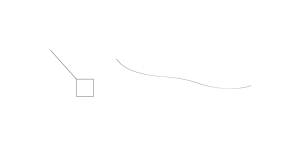
\includegraphics{fig/VFFD_pins}%300 dpi
  \caption{A CAD model design concept of a variable-friction floor tile coated with low-friction material and instrumented with sharp pins.%Reprinted with the author's permission.} %196 pins
  }
  \label{VFFD_pins}
\end{figure}

%Talk about the size of the pins? (don't think it's massively pertinent)
%"The size of the pins translates approximately to two classes of solution: sharp pins modify the macroscopic texture, similar to epoxy non-slip coatings, whereas large pins affect the microscopic texture, resulting in a perceived change of material."

A difficulty encountered in this instance is the selection of a material resilient enough to withstand human mass but that also has a low self-contact COF. For example, PTFE is relatively soft and susceptible to damage but offers a lower self-contact COF when compared with more robust materials, such as UHMWPE. In similar respects, an inherent limitation associated with the design is the natural erosion of the low-friction material due to the protruding sharp pins. Material replacement would have to be regularly performed to either the floor or shoe, whichever is nonactuated.

The concept is promising and could conceivably elicit a high degree of performance in terms of the range and resolution of achievable friction coefficients. Unfortunately, the design, manufacturing and maintenance drawbacks are less than favourable.


% 2. low-friction material and high-friction material with an elastic element.
\paragraph{High- and Low-Friction Materials}
\label{hlfmats}

The same authors propose a second material-based solution. Using both high- and low-friction materials on a single face of contact can be used to modulate friction by regulating the proportion of normal force experienced by both materials. This is done by controlling the position of one of the materials. In this case, the position of the high-friction material is controlled. To facilitate relative continuity in friction variation, an elastic element is placed between the high-friction material and position control element. The shoe sole face is composed of low-friction material and regions where the high-friction material may protrude. The design is such that when the elastic element is uncompressed (i.e., the high-friction material is not in contact with the floor), the friction experienced is that of the low-friction material. The concept is illustrated in Figure \ref{principle} \cite{millet2016design} and a prototype may be seen in Section \ref{VFSM}.

\begin{figure}%[tpb]
  \centering
  \includegraphics{fig/shoe_principle}
  \caption{A diagram illustrating the mechanism of the friction variation using high- and low-friction materials.}
  \label{principle}
\end{figure}

As described by Millet et al.\ \cite{millet2016design}, assuming Coulomb's model of dry friction and that the mass of the device is negligible with respect to a user's mass, the effective COF is described mathematically as follows:

% also taken directly from vf2.

\begin{align}
  F_\mathrm{human} &= F_\mathrm{lf} + F_\mathrm{hf}\\
  F_\mathrm{hf}    &= E_\mathrm{el} S_\mathrm{el} \varepsilon_\mathrm{el}\\
  \mu_\mathrm{eff} &= \frac{\mu_\mathrm{lf}F_\mathrm{lf}+\mu_\mathrm{hf}F_\mathrm{hf}}{F_\mathrm{lf} + F_\mathrm{hf}}\\
  \mu_\mathrm{eff} &= \mu_\mathrm{lf} + (\mu_\mathrm{hf} - \mu_\mathrm{lf}) \frac{E_\mathrm{el} S_\mathrm{el} \varepsilon_\mathrm{el}}{F_\mathrm{human}}\label{eq:mu}
\end{align}


$F_\mathrm{human}$ is the downward force applied by the user on the shoe sole. $F_\mathrm{lf}$ and $F_\mathrm{hf}$ are the ground reaction forces experienced by the high- and low-friction materials. $E_\mathrm{el}$ is the Young's modulus of the elastic element, $\varepsilon_\mathrm{el}$ its percentage strain and $S_\mathrm{el}$ its cross-sectional area, which is equivalent to the cross-sectional area of the high-friction material. The respective COFs of the high- and low-friction materials are $\mu_\mathrm{hf}$ and $\mu_\mathrm{lf}$. When the elastic elements are uncompressed (i.e., $\varepsilon_\mathrm{el}=0$), then $\mu_\mathrm{eff} = \mu_\mathrm{lf}$. Compression of the elastic element increases the force applied to the high-friction material $F_\mathrm{hf}$ by an amount equal to the decrease of force applied to the low-friction material $F_\mathrm{lf}$. If $F_\mathrm{hf}$ reaches the total force $F_\mathrm{human}$, the low-friction material is no longer in contact with the floor and $\mu_\mathrm{eff} = \mu_\mathrm{hf}$.

A number of issues present themselves if this design is used in a walking context. $F_\mathrm{human}$ and $S_\mathrm{el}$ will vary during stride due to varied gait styles. As such, the uniformity of spacing, surface area and proportion of high-friction material present at the contact face will play a role. For example, high-friction material should be present during heel strike and toe off phases of gait. The authors recommend using estimates of $F_\mathrm{human}$ and $S_\mathrm{el}$ as parameters for real-time friction control.

The methods discussed for modifying the materials present at the contact surface for variable friction represent viable and effective design concepts. The inherent drawbacks lie mainly in the realm of designing an effective and cost-conscious solution. Achieving extremely low COFs also remains an issue as both lubrication and rolling designs can elicit lower static COFs than PTFE in self contact.


% Rolling
\subsubsection{Rolling}

A number of implementations intended for free walking in virtual environments make use of rolling elements \cite{huang2003omnidirectional,schwaiger20072d}. Dimensionality plays a role in this design space as some implementations use 1D linear bearings or conveyor rollers to act as their low-friction mechanism, while others use omnidirectional BTUs or ball bearings to allow motion in 2D. Early designs of low- or variable-friction interfaces, used in locomotion studies, were 1D and either had no control mechanism \cite{pai1999induced} or simply kept their rollers locked or unlocked \cite{marigold2002strategies} and were thus only able to simulate two conditions: slippery and nonslippery. 

Millet et al.\ proposed the use of 1D conveyor rollers or 2D BTUs to be installed into floor tiles \cite{millet2011initial}. A control mechanism is presented for the conveyor roller, similar to the control mechanism presented in Section \ref{hlfmats}. A position control element determines whether high-friction material is in contact with the rotating elements, consequently setting the compressive strain of an elastic element located between the position control element and the material. While cost-effective, the design only allows for 1D variable friction \cite{millet2011initial}.

The 2D design arranged the BTUs in a uniform array on a tile while making use of a cover plate, seen in Figure \ref{BTU_CAD}, to avoid jamming of the edge of the foot during gait. Two forms of friction control are suggested, the first of which involves high-friction material, an elastic element and linear position control. The high-friction material would need to be actuated such that  it would come in contact with the ball of the BTU, either on its exposed face or by drilling a hole into its side, so as to resist rotation. The alternative is to place braking pins between the BTUs, whose protuberance is controlled. Both of the concepts are discussed in detail in Section \ref{mats}. The benefits of this method include low friction rendering capability and a potentially high degree of effectiveness. The main drawback is the complexity of design required to implement a control mechanism, which is largely imposed by spatial constraints \cite{millet2011initial}.

\begin{figure}%[tpb]
  \centering
  \setlength{\unitlength}{1mm}
  \begin{picture}(82,38)
    \put(20,0){\includegraphics[width=62mm]{fig/BTU_tile}}% 328 dpi
    \put(0,13){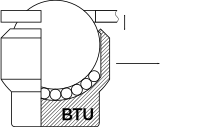
\includegraphics[width=25mm]{fig/BTU}}
  \end{picture}\vspace{-2mm}
  \caption{A CAD model of a conceptual 2D low-friction floor tile made of BTUs. Friction modulation may be done with braking pins between the BTUs or with a position controlled high-friction material mechanism described in Section \ref{mats}.%Reprinted with the authors permission.
  }
  \label{BTU_CAD}
\end{figure}

The key advantage with converting sliding friction to rolling friction is that it can achieve COFs as low as 0.03 \cite{millet2013vibration}. Unfortunately, there are a number of disadvantages associated with rolling designs. From a shoe based implementation perspective, steel rolling elements are heavy and would not make for a natural walking experience. In general, the limitations include friction anisotropy due to the spacing of the elements, vibrotactile noise, susceptibility to contaminants and difficulty in design and implementation of control mechanisms \cite{millet2016design}.

%Disadvantages: significant perceptual biases such as an uneven surface, vibrotactile noise,  and 
%- non-uniform surface (non-flat surface is what you mean)
%- difficult to control
%- heavy
%- easily subjected to contaminants
%- walking on steel in general is a bad idea, footwear is often made of soft, yet durable material. think about steel on marble or tile,  (Gabrielle's design does account for this), even so


\subsubsection{Vibration}
\label{vib}

% mech vib
With respect to HCI and hand interactions, vibration has been used considerably for friction modulation. Mechanical vibration, usually at ultrasonic frequency and micro-scale amplitude, is applied to a flat surface and a thin squeeze film of air is created when another object comes in contact with the surface, resulting in reduced friction \cite{winfield2007t,amberg2011stimtac}. The vibration can be simply and effectively controlled while offering an appreciable range of COFs. Piezoelectric actuators are commonly employed for this application  \cite{watanabe1995method,nara2001surface,biet2006piezoelectric,winfield2007t,amberg2011stimtac,levesque2011enhancing}, though voice coils and solenoids \cite{bau2010teslatouch} have also been used.

% mech vib - adv/dis
While effective and spatially compact, the portability of this technology remains to be established as these actuators require voltages much higher than what is commonly found in mobile device batteries. Additionally, mechanical actuators are generally spaced about the periphery of the interaction space for these devices, making mechanical actuation less suitable for large areas as the amplitude of vibration will decrease for locations further away from the actuators. Attenuation of frequencies will also vary when using mechanical vibration due to the resonant frequency of the vibrating plane material \cite{bau2010teslatouch}. Using vibration in a walking context remains a question as both the surface area of feet and mass of humans are at least two orders of magnitude greater than that of the finger, thus, porting the technique to floor-based methods is unlikely to scale up \cite{millet2016design}.

% elec vib
A more recent innovation in vibration-based variable friction, Bau et al.\ created variable-friction devices employing \textit{eletrovibration} \cite{bau2010teslatouch} and \textit{reverse electrovibration} \cite{bau2012revel}. Electrovibration involves applying an oscillating voltage signal to a conductive surface. When a dry finger comes in contact with the surface, a periodic attraction force is seen between the surface and the finger, which is perceived as a ``rubbery sensation" when the finger is in motion. The explanation for this phenomena is that the dry skin acts as a dielectric layer between the conductive screen and fluid inside of the finger, analogous to the principle of operation of a capacitor \cite{mallinckrodt1953perception}.

% elec vib - adv/dis
Unfortunately, electrovibation only works for bodies in motion, thus, there are no noticeable effects for actions performed on the screen at a point (e.g., button pushes, press and hold actions). In addition, reverse electrovibration requires common grounding for each object in the interaction, presenting clear mobility limitations. Passive instrumentation must also be applied to an object to be used with this technology, though, little maintenance is required following this. Electrovibration offers a greater frequency range and much more uniform response characteristics in comparison to mechanical vibration. The portability of the technology is far greater than that of its mechanical counterparts, requiring a small battery and circuit board for implementation \cite{bau2010teslatouch,bau2012revel}. In relation to a walking context, the aforementioned limitations are of less concern as an augmented floor can easily be grounded and the benefits of the method, if applicable to walking, are quite enticing. Future work may include confirming the viability of scaling this technology to a walking context and perhaps determining the range of renderable COFs.


\subsection{Applied Variable Friction}


We commonly see haptic feedback employed to enrich perceptual experiences by better engaging a user or by communicating through a less congested or more private feedback channel (e.g., button touches, message notifications). Variable friction is a subset of this area. As mentioned earlier, common HCI applications of variable friction include augmented pointing performance, usability and user experience. With respect to pointing, high-friction target regions can assist users by making targets ``sticky", while the remainder of the interaction space is low friction. This results in reduced overshoot and simplified fine motor control when pointing. Friction modulation can also add an extra dimension of navigation and tactility when performing common tasks such as drag and drop actions or using widgets and sliders. Levesque et al.\ \cite{levesque2011enhancing} confirmed these presumptions\dan{replaced "confirmed these postulates" with "confirmed these presumptions"}, specifically to touchscreens, by evaluating variable friction against constant friction while including distracting targets. This concern may arise during the design of a user interface that makes use of a pointer, as pointing trajectories are likely to become occluded by the high-friction effects of other potential targets. The interface modality was then tested with four common applications (i.e., alarm clock, file manager, game, text editor) where user evaluations gave indications of better awareness of system state, as well as augmented realism and experience \cite{levesque2011enhancing}.

Bau et al.\ introduced some novel ideas to the variable-friction design space that have yet to be explored. They propose personalized and private feedback for use in public interfaces (e.g., ATMs, public transit kiosks, library kiosks), which may include tactile hints for forgotten passwords as well as user-defined shortcuts and themes. Also mentioned is the potential for navigational guidance for the visually impaired (i.e., following a textured path along a wall, screen or floor) and use of the technology as an ``internal ambient information display" (e.g., time-based reminders, notifications) \cite{bau2012revel}.


\subsection{A Variable-Friction Shoe Mechanism}
\label{VFSM}


Foot-based interfaces with focus on controlled friction variation are uncommon in the literature \cite{millet2016design} but can be found on the retail market\dan{replaced "see commercial exposure" with "can be found on the retail market"}.\footnote{\url{http://www.heelys.com/}} In the preceding sections, the majority of designs and concepts are extrinsically sensed and actuated, meaning that the friction variation occurs in a specific environment (i.e., touchscreen, floor). Extrinsic designs are spatially confined and require specialized, instrumented infrastructure making design and implementation difficult and expensive. The ideal solution is a ubiquitous, intrinsically sensed and actuated one that is free from the requirement of specialized infrastructure (e.g., an instrumented shoe). Bau et al.\ addressed this problem well with REVEL \cite{bau2012revel} and the Shared Reality Lab has actively sought out a ubiquitous and self-contained solution \jer{intrinsic to what?} \dan{Referring to an intrinsically sensed and actuated variable-friction platform, replaced "intrinsic" with "self-contained"} with varied approaches \dan{Modified the ending of the sentence to be more explicit, i.e., an intrinsically sensed and actuated variable-friction shoe} \cite{millet2016design,king2014development,robert2016development}.

The friction-varying device used in this work is a braking mechanism small enough to fit inside of a shoe sole, designed and fabricated at the Shared Reality Lab in 2013~--~2014. Figure \ref{mechanism_fiducial} shows an annotated picture of the mechanism. Friction variation is performed using the method described in Section \ref{hlfmats}. A set of brake pads, composed of a rigid element (aluminum), elastic element (EVA foam) and high-friction material (Santoprene rubber), are translated orthogonally with respect to the shoe sole to modulate friction. The surface area of the Santoprene was 1,140~mm$^2$ and the thickness of the EVA foam was 7~mm. The actuator driving the brake pads was a thin-profile stepper motor. Rotational motion from the motor is transferred by a gear train to two lead screws, which are fastened by thread on to the rigid element of the brake pads. A lead screw is a simple linkage that converts rotational motion into translational motion. Figure \ref{leadscrew_closeup} shows a close-up view of the lead screw to illustrate and clarify this explanation. On the bottom of the mechanism, PTFE tabs protrude as the supporting low-friction material \cite{king2014development}.

% SA = 1,140 mm^2 =(20x30, 45x12)
% EVA foam thickness ~= 7 mm

% Mechanism pictures with annotations
\begin{figure}%[tpb]
  \centering
  \includegraphics[scale=0.1]{fig/mechanism_fiducial}
  \caption{The top image shows the mechanism with the brake pads attached. The bottom image shows the mechanism with the brake pads detached to highlight the gears and lead screws.}
  \label{mechanism_fiducial}
\end{figure}


% Close up view of a lead screw
\begin{figure}%[tpb]
  \centering
  \includegraphics[scale=0.12]{fig/leadscrew_closeup}
  \caption{A close up view of a lead screw.}
  \label{leadscrew_closeup}
\end{figure}


\section{Human-Centred Approaches in Slipperiness Measurement and Psychophysics}

%discrimination thresholds

This section highlights the importance of evaluating human perception of sliding friction and discusses the use of psychophysical methods to accomplish this.

\subsection{Human-Centred Approaches}

Human-centred approaches for evaluating slipperiness are necessary for their use in developing research hypotheses and models for the prediction of workplace risks caused by slips and falls. The approaches are used as alternatives to, or to validate apparatus-based friction measurements \dan{explanation added to clarify what human-centred approaches are used as alternatives to}. There are three such approaches applied to determining slipperiness: objective, subjective and combined. Objective approaches measure ground reaction forces, utilized friction,\footnote{\textit{Utilized friction} is defined as the friction force required to maintain motion. \textit{Available friction} refers to the friction coefficient at which slippage is likely to occur. Utilized friction should not exceed available friction for unperturbed walking. Mathematically, utilized friction is defined as the ratio between shear force on the shoe sole and vertical downward force.} body kinematics during slip, centre of mass trajectories and electromyographic activity of muscles during compensation. Subjective approaches use paired comparisons of footwear and floor surfaces, measure slip perception and have rating scales for balance and safety. Combined approaches use metrics from both \cite{gronqvist2001human}. While practical, there are drawbacks to human-centred approaches such as variance, which arises from experimental bias \cite{jung1993methods}. In addition, experimentation is generally done in a laboratory setting, making field applications rare and repeated tasks are often used, which have learning or carryover effects that affect measured outcomes \cite{gronqvist2001human}.


\subsection{Psychophysical Methods}

%Psychophysical methods to haptics
To characterize our hardware, we set our attention on the discipline of psychophysics, which is concerned with relating physical stimuli to human perception. Psychophysical methods are used to determine discrimination thresholds otherwise known as just noticeable differences (JND). A JND is the minimal difference between two stimuli that leads to a change in perception. The threshold is considered as the stimulus difference that will be detected at a fixed percentage of a number of trials, typically around 75\% \cite{treutwein1995adaptive}. We make use of psychophysics to determine human sensory resolution with respect to sliding friction in this specific case. There exist a number of studies that apply combined human-centred approaches of slipperiness and psychophysics to evaluate friction perception  \cite{lanshammar1985assessment,cohen1994psychophysical,gronqvist1993slipperiness,samur2009psychophysical,bau2010teslatouch}.

%23 tiles total
Cohen and Cohen~\cite{cohen1994psychophysical} performed a psychophysical assessment on the perceived slipperiness of floor tiles. A slipperiness comparison, where subjects slid their bare foot on a reference tile and a test tile, was done. Subjects indicated which tile was more slippery and were also asked which mechanisms they used to assess the slipperiness of a tile, the most popular of which was said to be the sliding resistance. Results of the experiment were conflicting \jer{word choice; implies that the results came in bursts?} \dan{Agreed, replaced "sporadic" with "conflicting"} and did not consistently agree with measured COFs (i.e., subjects often indicated that the more slippery tile offered greater sliding resistance, or vice versa) \dan{modified as warranted}.

A second investigation had subjects rank seven tiles in terms of their slipperiness using isolated visual, auditory and tactile feedback modes. This information was collected to better understand how humans perceive floor slipperiness as the varied results in the first experiment suggested that visual and auditory cues have the ability to override tactile ones and influence perception. The study concludes that under experimental conditions, tactile cues are the most accurate tool that humans have in determining relative levels of slipperiness, despite their lack of accuracy \cite{cohen1994psychophysical}.

%The information obtained was used to determine JNDs for the range of COF's the interface could produce. 
Samur et al.\ and Bau et al.\ measured the haptic rendering capabilities of their respective variable-friction tactile interfaces, in terms of friction JNDs, using adaptive staircase methods. Friction discrimination experiments were carried out where subjects were presented with two stimuli sequentially. One of the stimuli is a reference value and the other is modified based on a subject's perception until a point of convergence has been reached. Both comparisons were done by sliding the pad of the index finger back and forth on the respective variable-friction interfaces \cite{samur2009psychophysical,bau2010teslatouch}.

%The study concluded that the average JND for the COF of the interface, in terms of a Weber fraction, was 18\%.


\section{Pointing Evaluation and Foot-Controlled Pointing}

In this section we will discuss the metrics associated with pointing performance evaluation and review foot-controlled pointing in general.

\subsection{Pointing Evaluation} % perhaps an appendix piece.
\label{pointing_eval}

Despite efforts by academia and industry \cite{soukoreff2004towards} the evaluation of pointing performance in HCI remains to be universally standardized. The following explanation of pointing performance evaluation is based off the work of Soukoreff and MacKenzie \cite{soukoreff2004towards}. Their objective was to improve the comparability and consistency of experiment conditions or movement time prediction, using the ISO 9241-9 standard, in the evaluation of pointing devices.

When evaluating the performance of a pointing device, a predictive model of human movement time known as Fitts' Law \cite{fitts1954information} is applied. The Shannon formulation of Fitts' Law will be described here. The original Fitts' paradigm uses a 1D horizontal arrangement while the ISO standard utilizes a 2D circular task. The layouts of these pointing tasks can be seen in Figure \ref{1D_2D}.


\begin{figure}[tpb]
  \centering
  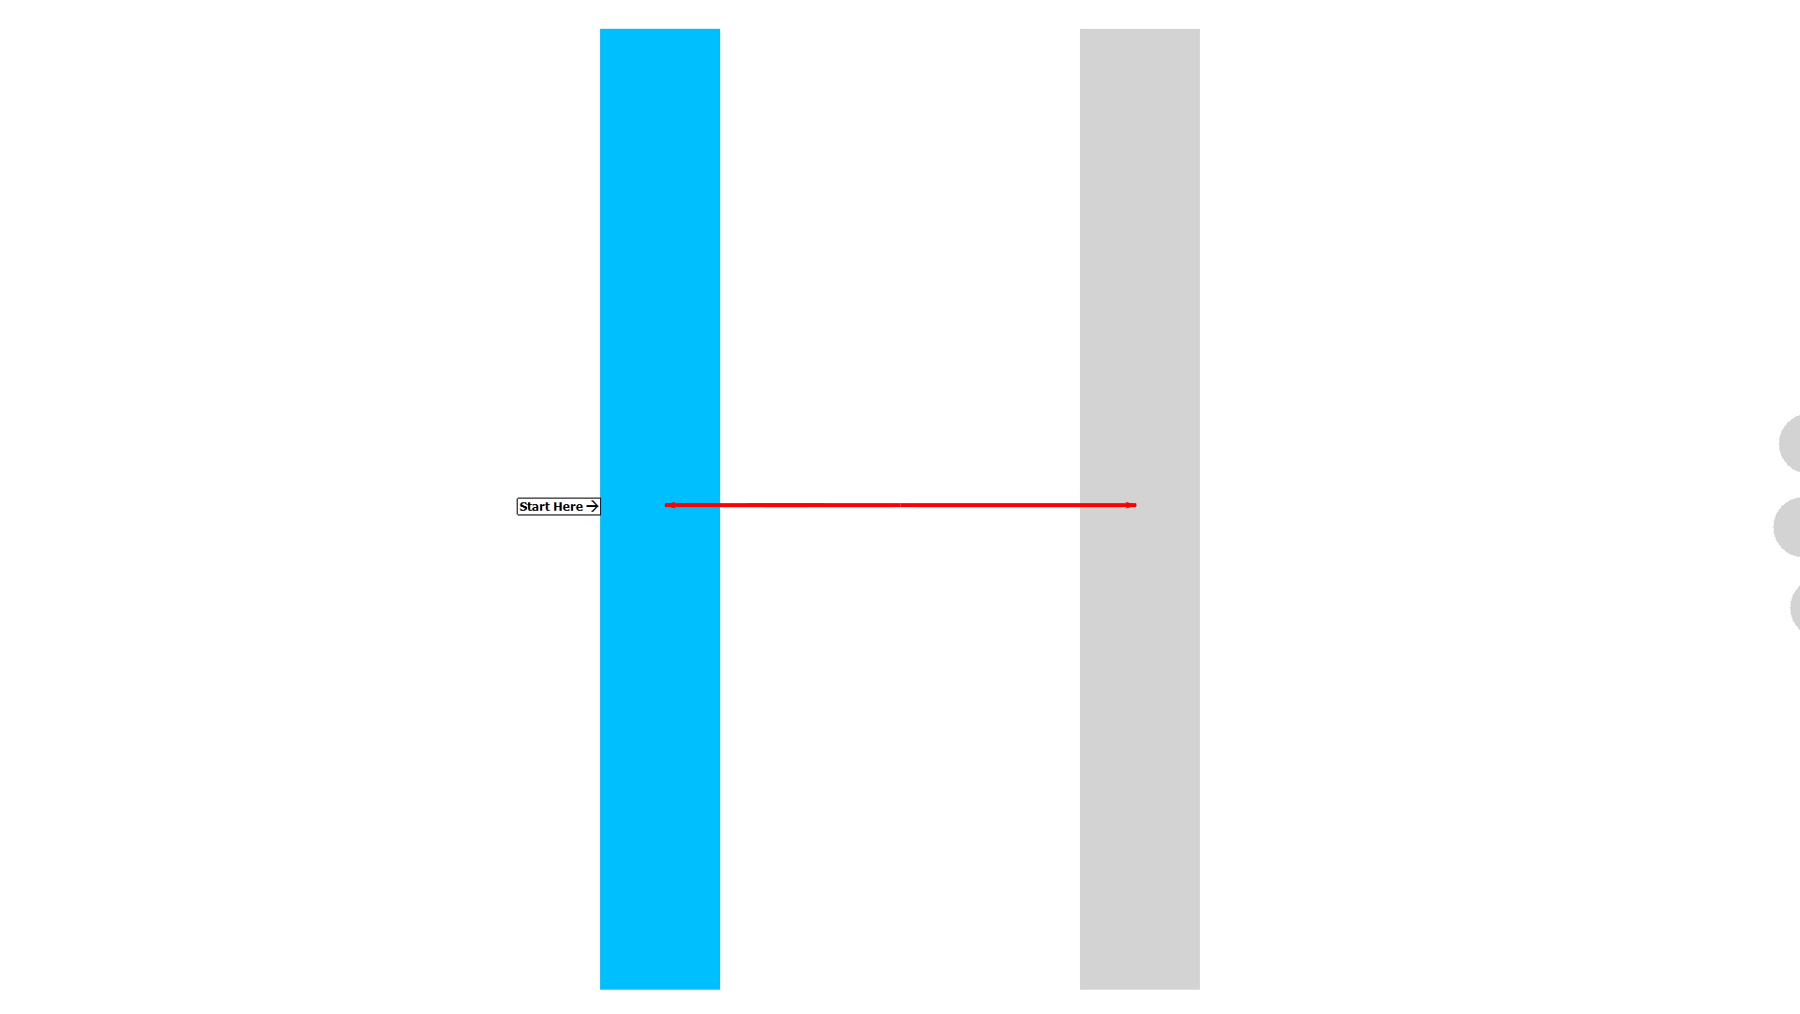
\includegraphics[scale=0.2]{fig/1D_2D}
  \caption{On the left, the original 1D Fitts' task is seen. On the right the 2D ISO 9241-9 task layout is seen. Subjects click in sequence in the patterns indicated by the red arrows during each movement condition.}
  \label{1D_2D}
\end{figure}


Mathematically, Fitts' Law is described as follows:

\begin{align}
	MT = a+b\times{}I\!D
\end{align}

Here, \textit{MT} is the predicted movement time of the model, in seconds. The parameters \textit{a} and \textit{b} are determined by running a linear regression on the performance data. \textit{ID} is the index of difficulty of the pointing task, described by the following:

\begin{align}
	I\!D = log_{2}\bigg(\frac{D}{W} + 1\bigg) \newline{}
\end{align}

The unit of the \textit{ID} is bits. Here, \textit{D} is the centre-to-centre distance from the previous target (i.e., pointer starting position) to the current target centre and \textit{W} is the width or diameter of the target, both in pixels.

A number of different target widths and distances are selected for pointing device characterization. Each combination of distance and width is referred to as a movement condition. Movement conditions are selected such that an appreciable range of \textit{ID}s are tested. Commonly, the range lies between two and six bits. Each movement condition is presented to subjects a number of times, usually around fifteen. A number of parameters are recorded during experimentation, including: movement time, movement distance, error rate (the percentage of missed targets) and end-point scatter data (the distance between the target centre and actual click). End-point scatter data and movement distance are recorded to apply the adjustment for accuracy, which involves a recalculation of the \textit{ID}, here referred to as the \textit{effective} index of difficulty (\textit{IDe}):

\begin{align}
	I\!De = log_{2}\bigg(\frac{De}{W\!e} + 1\bigg) \\
	W\!e = 4.133\sigma{}
\end{align}

The standard deviation ($\sigma$) of the end point scatter data is used to find the \textit{effective} width, while the \textit{effective} distance is calculated as the mean movement distance from the beginning point of movement to the end point.

The effective indices are calculated to improve the accuracy of the movement time model. The exact target widths and distances are what we ideally wish to measure movement time and error rates over, but invariably, human error will come into play. Specifically, movement end-point data is not likely to adjust to specified target widths, thus there will be inconsistency in error rates with respect to their \textit{ID}s. Additionally, it has been found that subjects perform slower on lower \textit{ID}s and will not move to the target centre once the target region has been reached \cite{soukoreff2004towards}. Applying the adjustment for accuracy accounts for these issues and offers a more accurate \textit{ID}.

Each subject will produce \textit{n} ordered pairs of \textit{IDe} and \textit{MT}, where \textit{n} is the number of movement conditions. For clarity, \textit{MT} in this instance is the mean movement time of a condition. Once a suitable number of subjects have been evaluated, a least-squares linear regression is performed on this data to find the aforementioned parameters, \textit{a} and \textit{b}:

\begin{align}
	MT = a+b\times{}I\!De
\end{align}

The predictive model of movement time for the device is:

\begin{align}
	MT_{predicted} = a+b\times{}I\!D
\end{align}

\ilja{The explanation of the dependent measure throughput (P19) is too sparse to expect a reader to understand its meaning and interpretation. It would be good to add a little bit of background information.}

\dan{Added below.}

For the purpose of comparing experiment conditions, a performance measure known as throughput (\textit{TP}) is calculated. \textit{TP} is considered a complete measure because of its consideration of both speed (\textit{MT}) and accuracy (\textit{IDe}). \textit{TP}, as described by Fitts' himself, ``The average rate of information generated by a series of movements is the average information per movement divided by the time per movement" \cite{fitts1954information}. Thus, \textit{TP} is defined as: \jer{this is better, but could still go further in explaining what throughput is actually measuring.  See the Wikipedia definition (under Fitts' Law) of IP, for example}

\dan{Further elaboration added, and in the next paragraph}

\begin{align}
	TP = \frac{IDe}{MT}
\end{align}

\textit{IDe} is used in this calculation as it better describes the actual movements that subject's performed rather than assuming the movements were performed as desired. Each movement condition has an associated \textit{TP}, which Fitts' Law assumes to be relatively constant over all amplitudes and widths. To find the \textit{TP} of a pointing device, the mean \textit{TP} of all movement conditions over all subjects is calculated. This considers the effects of both the slope and intercept parameters of the linear regression model into a single metric, which facilitates comparisons across various movement conditions and device studies. To test the significance of \textit{TP}s, a repeated measures ANOVA is used. The \textit{TP} of a device is calculated as:

\begin{align}
	TP = \frac{1}{m} \sum_{i=1}^{m} \bigg( \frac{1}{n} \sum_{j=1}^{n} \frac{I\!De_{ij}}{MT_{ij}}  \bigg)
\end{align}

In the above instance, \textit{n} represents the number of movement conditions and \textit{m} represents the number of subjects evaluated, thus \textit{TP} is calculated as a mean of means.

%\textit{TP} is considered a complete metric for pointing as it incorporates both speed and accuracy when the \textit{IDe} is used in its calculation.

We use Fitts' Law to evaluate and characterize a novel pointing device. Rather than estimating movement times, a number of movement times are measured and their associated \textit{IDe}s are used to estimate the mean \textit{TP} for the device. The pointing device may then be evaluated for a set of movement conditions in various modalities (e.g., variable friction vs.\ constant friction) to determine their effects on the Fitts' model and \textit{TP}.


\subsection{The Foot as a Pointing Device}

The foot has been studied from an HCI perspective as early as the 1960s \cite{english1967display}. Early work sought out an ideal ergonomic and functional design of foot-controlled interfaces intended to augment pointing performance and experience in the desktop environment \cite{english1967display,pearson1986moles,pearson1988exploratory}. The common keyboard and mouse configuration presents a clear lack of efficiency when both cursor positioning and text entry are required. Given a comparison of dexterity between the fingers and toes, it appears obvious that the hands are better suited to focus mainly on the keyboard \cite{pakkanen2004appropriateness}, thus; early research into foot control focussed on cursor control. This remains a popular topic in the field as the root issue has yet to be solved. Nevertheless, foot-controlled interfaces have seen a wide application range including: mode selection, spatial navigation, mobile phone control, command activation, gaming, tempo selection, user identification and text input, as highlighted by Velloso et al.\ \cite{velloso2015interactions}.

\begin{table}[]
\centering
\caption{A table summarizing reported throughputs and error rates of hand and foot-operated pointing devices evaluated using ISO 9241-9. If a range of values is indicated, the ends of the interval represent the minimum and maximum throughputs reported over multiple evaluations. Note that in Velloso's work \cite{velloso2015interactions}, a depth camera was used to track foot motion for the foot-controlled devices. No foot-controlled depth cameras were used.}
\label{ISO_comparison}
\begin{tabular}{@{}l|ll@{}}
\toprule
\textbf{Hand-Controlled Pointing Device}          & \textbf{Throughput (bits/s)} & \textbf{Error (\%)} \\ \midrule
Mouse \cite{soukoreff2004towards}                 & 3.7~--~4.9                   & 11                \\
Trackball \cite{soukoreff2004towards}             & 3                            & 8.6               \\
Touchpad \cite{soukoreff2004towards}              & 0.99~--~2.9                  & 7                 \\
Wiimote \cite{natapov2009iso}                     & 2.59                         & 10.2              \\
Joystick \cite{soukoreff2004towards}              & 1.6~--~2.55                  & 9.6               \\
Wii Classic Controller \cite{natapov2009iso} 	  & 1.48                         & 6.58              \\ \midrule
\textbf{Foot-Controlled Pointing Device}          & \textbf{Throughput (bits/s)} & \textbf{Error (\%)} \\ \midrule
Depth Camera \cite{velloso2015interactions}      & 1.16                         & 7.64              \\
Depth Camera (1D) \cite{velloso2015interactions} & 1.75                         & 8.43              \\ \bottomrule
\end{tabular}
\end{table}

Table \ref{ISO_comparison} highlights a clear performance disparity between the hand and foot in tasks of equivalent complexity. Both movement time and accuracy play a role in this disparity as it takes the foot much longer to make precise movements  \cite{pakkanen2004appropriateness}. The foot generally takes about twice as long as the hand to complete an equivalent movement  \cite{hoffmann1991comparison}. This prompted researchers to simplify the actions done by the foot such that performance may approach that of hand-controlled devices. Task simplification narrowed interaction types to simple gestures (e.g., medial/lateral heel rotation, dorisflexion, plantar flexion) and further constrained peripherals to devices such as pedals or switches. Consequently, the input bandwidth was narrowed, especially in terms of accuracy and applications involving menu selection and non-accurate spatial tasks were seen. Acceptable performance in terms of speed and accuracy were found in these contexts, validating that the feet at least have a place in HCI for simplified tasks  \cite{pakkanen2004appropriateness,scott2010sensing,zhong2011foot,simeone2014feet}.

While task simplification is effective, it oversimplifies the capabilities of the foot. The feet commonly perform a number of complex tasks such as driving, gear shifting, biking, organ/piano playing, guitar effects modulation and in sports such as soccer. Garcia and Vu compared the performance of a hand-controlled trackball and a foot-controlled mouse in word processing tasks over ten sessions to investigate the effects of learning. Trackball performance was superior, but performance quickly reached a plateau. Foot mouse performance continually improved over the sessions suggesting an inherent bias in a comparison between hand and foot-operated pointing devices due to experience with hand pointing. It also suggests that further practice may help to meet or exceed conventional mouse pointing performance, necessitating further research on the topic \cite{garcia2011effectiveness,velloso2015feet}.

Foot pointing devices include similar peripherals as their hand-controlled counterparts (e.g., joystick, trackball, mouse) \cite{springer1996position,pakkanen2004appropriateness,ye2005shoe}. Early prototypes varied as English et al.\ approached the problem using a knee lever \cite{english1967display}, while Pearson and Weiser presented their mechanically intricate mole designs \cite{pearson1988exploratory}.

\ilja{The definition of extrinsic devices is not explicit enough. While it's workable on page 13, it is less clear on page 21 when discussing how "colour" and "depth" are supposedly extrinsic. In addition, extrinsic is used in combination with "design", "methods", and "sensing", which adds to the confusion.}

\dan{Added below. Just to note, the reason for the separate citations at the end of the following paragraph is because I am meaning to cite "velloso2015feet" for the entire paragraph, this seemed the most appropriate way to do so.}

%"Extrinsic sensing refers to when the feet are tracked through sensors placed on the environment." \cite{velloso2015feet}

In the literature, there are three methods used to sense foot input: mediated, intrinsic and extrinsic. Mediated sensing records the movements of devices operated by the feet (e.g., pedals, foot switches and balance boards). Intrinsic sensing methods make use of sensors attached directly to the feet, while extrinsic sensing places sensors around the interaction space to track the feet. Intrinsic sensing, usually in the form of wearables or even mobile devices \cite{scott2010sensing}, track the foot using accelerometers, gyroscopes and hall effect sensors \cite{ye2005shoe,velloso2015interactions}. Extrinsic methods make use of colour \cite{paelke2004foot}, depth \cite{simeone2014feet} and motion capture \cite{kume1998foot} cameras, as well as rotation and force sensor instrumented devices and floors \cite{visell2010interaction}. Binary input (i.e., mouse clicks) for foot-controlled input devices is generally taken from force sensors \cite{visell2010interaction}, IR reflective sensors \cite{ye2005shoe}, textile switches \cite{laviola2001hands} and even the conventional mouse \cite{velloso2015interactions}~\cite{velloso2015feet}.


\chapter{A Variable-Friction Prototype Shoe and its Characterization}
\label{design_characterization}

% TABS - refers to the Teflon ridges protruding from the edges of the mechanism
% PADS - refers to the brake pads

In this chapter, we describe the process of designing and characterizing a variable-friction prototype shoe.

\section{Design}
\label{design}


\subsection{Mechanical}

The prototype used in this work is a device that attaches to one's shoe sole and can vary the COF experienced by the wearer in a controlled manner. The mechanism enabling variable friction is described in Section \ref{VFSM} and was to be installed onto the heel of a shoe sole, which led to the design of a prototype. Ensuring the longevity of the mechanism was a priority, especially given the manufacturing time and effort. As such, the device was not to be subjected to the rigours of walking initially. Force, on the order of magnitude of human weight, applied to the PTFE tabs would result in high stress on the PTFE, which may lead to significant deformation or even breakage of the tabs in a short period of time.

The prototype, seen in Figure \ref{prototype_fiducial} with annotations, was to be used strictly in low-stress scenarios. As such, it was decided that the sole would be kept flat since it would be used in sliding contexts. The mechanism was fastened near the edge of a rounded rectangular wood plate whose width is slightly greater than that of the mechanism itself. A block, of equal thickness and similar shape as the mechanism, was affixed at the opposing end of the plate. The bottom face of the block was coated with a layer of PTFE. To fasten the prototype to a shoe, the elastic mesh from a pair of Yaktrax\textsuperscript{\textregistered}\footnote{\url{http://www.yaktrax.ca/}} was used. The mesh forms around a smaller plate fastened to the opposing face of the main rounded rectangular plate. The mesh plate is separated from the larger main plate by seven shims, such that the elastic mesh may be manipulated to a wearer's preference. This allows for a range of shoe sizes to be used, facilitating accommodation to a variety of subjects in experimentation. To achieve closed-loop brake pad position control necessary for the experimentation in Chapter \ref{foot_pointing}, a rotary encoder with a gear was mated with the mechanism's gear train. The encoder itself was adhered to the bottom face of the mesh plate. A rectangular hole was made in the main plate to fit this. 

\begin{figure}[tpb]
  \centering
  \includegraphics[scale=0.085]{fig/prototype_fiducial}
  \caption{Top, side and bottom pictures of the prototype with annotations.}
  \label{prototype_fiducial}
\end{figure}


\subsection{Electronics} 

As described in Section \ref{VFSM}, friction is modulated by controlling the extension of the mechanism's brake pads. A stepper motor, mechanically connected to the brake pads, is driven by a motor driver chip. For the experimentation described in Section \ref{characterization} and Chapter \ref{perception}, brake pad position was open-loop-controlled as the pads were free from external loading during actuation. The motor was driven at low speed in a microstepping mode in these instances to ensure accurate positioning \cite{baluta2007microstepping}. Closed-loop position control was necessary for the experimentation done in Chapter \ref{foot_pointing}, as the brake pads were under load during actuation. Brake pad extension was tracked by an encoder sensing the rotation of the gear train. The encoder and driver chip were connected to a microcontroller development board, which received brake pad extension commands via USB. Table \ref{elec_table} details the principal components of the system.

%The current waveforms sent to the motor are sinusoidal, thus reducing step-to-step mechanical oscillations and velocity ripple.

\begin{table}[]
\centering
\caption{Main electronic components of the prototype.}
\label{elec_table}
\begin{tabular}{@{}l|lll@{}}
\toprule
\textbf{Component} & \textbf{Manufacturer} & \textbf{Model Number} & \textbf{Miscellaneous}          \\ \midrule
Motor              & Moon's Industries     & 23HM6401              & \textgreater~300 RPM max. speed \\
Motor Driver       & Pololu                & A4988                 & 1.5 A max. current   \\
Rotary Encoder     & Broadcom Limited      & HRPG-ASCA\#16C        & 120 CPR           \\
Microcontroller    & Sparkfun              & Arduino Pro Mini 328  & 5 V, 16 MHz                     \\
Power Supply       & Mean Well             & S-350-27              & 24 V, 13 A                      \\ \bottomrule
\end{tabular}
\end{table}


\section{Characterization}
\label{characterization}

To gain insight as to the surfaces the prototype could potentially emulate, the range of static COFs the prototype could render were determined. The static COF was selected since the dynamic COF of PTFE rapidly increases as velocity increases \cite{Dupont1996}, making it significantly more difficult to accurately characterize without gaining further information .


\subsection{Method}

The static COF rendering capabilities of the prototype were characterized by performing a simple ``tilt and slide" test. The prototype was placed on a level PTFE-coated piece of wood, which was slowly tilted about one of its edges until the prototype began to slide. The tangent of the angle at which sliding occurs defines the static COF ($\tan\theta=\mu_s$). To gain a clear understanding of the prototype's behaviour, mass and brake pad extension were varied in these tests. Their respective distributions were spaced equally over 11.4~kg and 4.4~mm ranges. Five masses $\times$ eight brake pad extensions $\times$ ten repetitions per condition, resulted in 400 trials in total. The brake pad extension of the prototype was held constant throughout each set of trials while the mass was incrementally increased over the tested range. After each set of trials was completed for a specific brake pad extension, the PTFE surface and prototype sole were sanded with 600 and 1000 grit sandpaper and subsequently cleaned with isopropyl alcohol.  This was done to ensure surface consistency between trials as PTFE deforms when abrasion occurs and tends to flake, which results in self lubrication.


\subsection{Apparatus and Procedure}

The PTFE surface was laid flat on the floor having one of its edges flush with a piece of tape to restrict any sliding motion. The opposing edge of the surface had an eyelet fastened to its centre. A piece of Kevlar\textsuperscript{\textregistered} string ran through the eyelet to a hand-controlled crank clamped to a table above the surface. Kevlar\textsuperscript{\textregistered} string has an extremely low extensibility, around 2\%, hence its selection \cite{Dupont2000}. To facilitate smoother motion, a piece of PTFE was affixed at the table's edge where the string made contact, due to the placement of the crank. To detect the moment at which sliding began, another piece of string was taped across the surface and used as a marking tool. The rear edge of the heel of the prototype was positioned such that it was in contact with the string at the beginning of each trial. The various masses were firmly secured inside of a boot fastened to the prototype. A trial was performed by slowly turning the hand-controlled crank, which wound the Kevlar\textsuperscript{\textregistered} string and thus increased the inclination of the surface. To improve estimation accuracy for the onset of sliding, a slow tilting rate reduced the influence of human visual perception reaction time. The moment at which the experimenter noticed the prototype's heel separating from the orange marking string, cranking was ceased and the height of the edge of the surface having the eyelet was measured using a Vernier caliper and laser range finder.\footnote{\url{http://www.bosch-pt.com/productspecials/professional/dle50/au/en/start/index.htm}} Figure \ref{tilt_apparatus_fiducial} illustrates the setup.

\newpage

\begin{figure}[tpb]
  \centering
  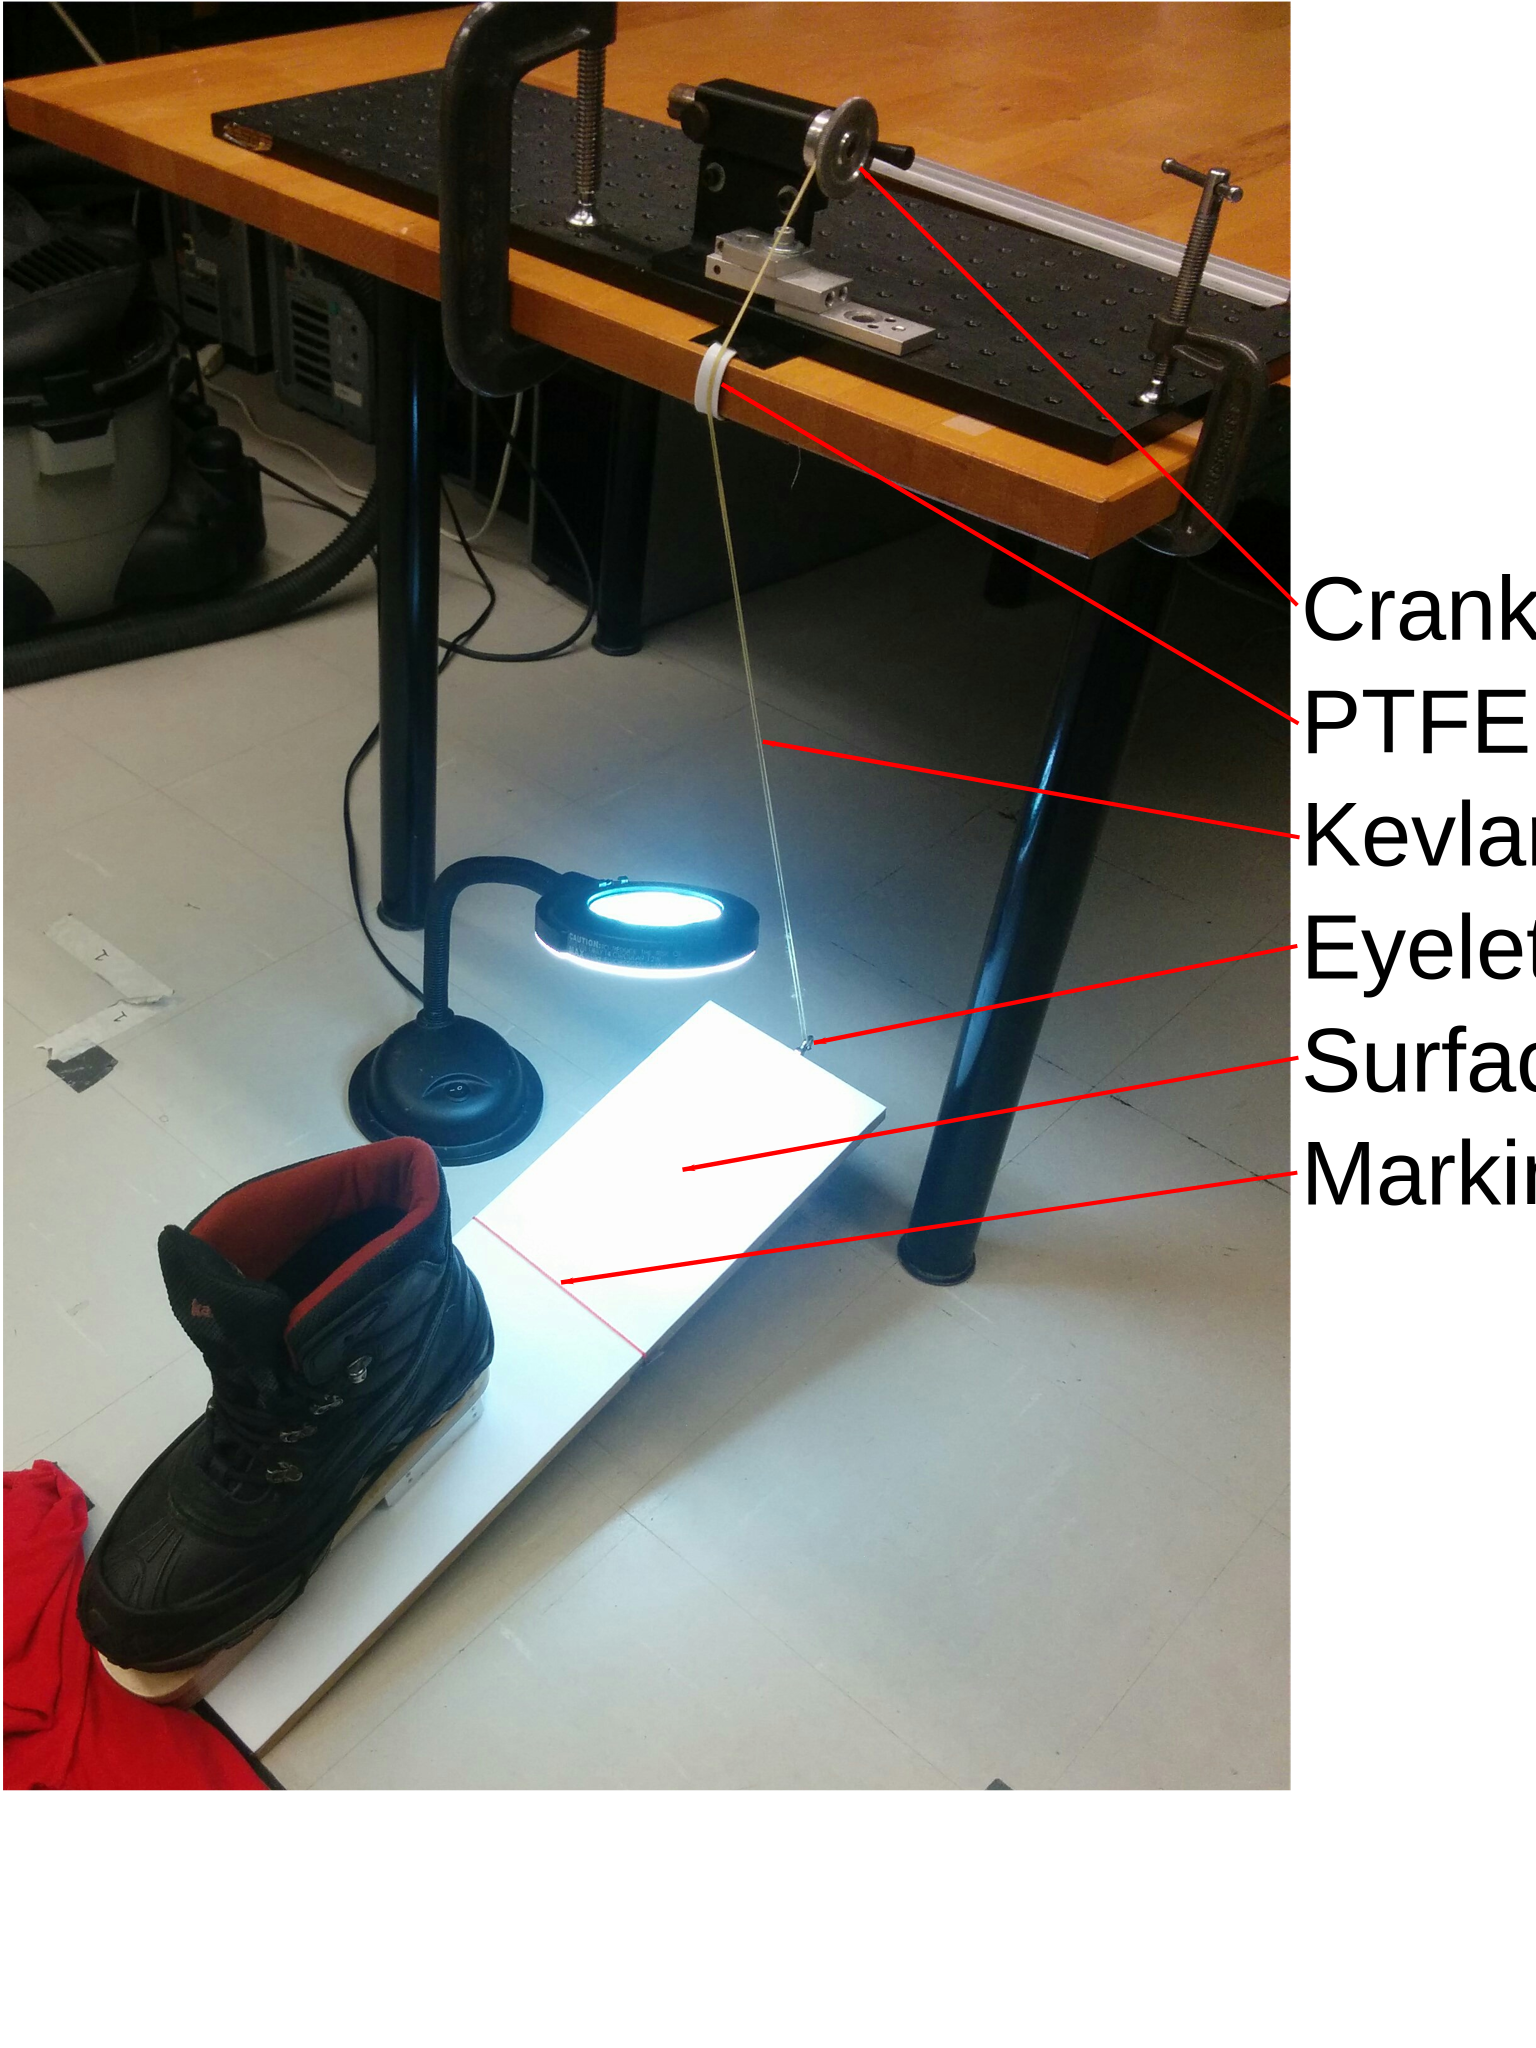
\includegraphics[scale=0.1]{fig/tilt_apparatus_fiducial}
  \caption{Tilt and slide test apparatus with annotations.}
  \label{tilt_apparatus_fiducial}
\end{figure} 

\subsection{Results}

Despite a lack of electronic control, the results indicate a well-controlled experiment. The expected behaviour of the onset of slipping is observed.

\begin{figure}[tpb]
  \centering
  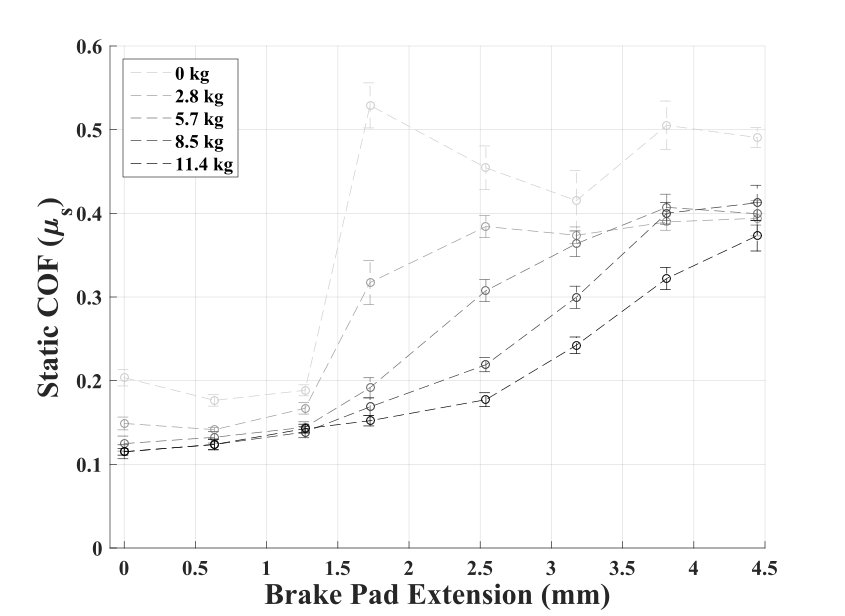
\includegraphics[scale=0.6]{fig/COF_vs_BPE}
  \caption{The static COF of the prototype at various masses and brake pad extensions. Error bars correspond to a single standard deviation.}
  \label{cof_vs_bpe}
\end{figure}

Figure \ref{cof_vs_bpe} shows the results from the tilt and slide test. Relative consistency is seen over the range of masses tested in terms of the COF at minimum and maximum brake pad extensions. When the prototype is left massless or lightly loaded, the COF characteristic becomes binary and a reduction in consistency is seen. Binary behaviour is expected as the EVA foam compresses less at such pressure levels. Thus, a considerably reduced proportion of the normal force is experienced by the PTFE of the prototype. In the subset of cases where the brake pad was considerably extended, the brake pads physically raised the prototype as the pressure was not enough to compress the foam. As such, the PTFE tabs of the mechanism were not in contact with the surface. Reduced consistencies are explained by slight perturbations in tilting rate due to a hand-cranked setup, resulting in variance of the proportion of normal force on the PTFE and brake pads. It is clear that as mass is increased, the concavity of the trend defining the static COF varies from concave down to concave up. The concave down behaviour is explained by the low-loading cases. Overall, this trend illustrates a decreased COF with increased pressure, which is in agreement with other PTFE COF characterizations \cite{Dupont1996}. When appreciable load is applied, the prototype COF characteristics exhibit improved consistency as the foam cannot raise the prototype under such conditions, resulting in a greater proportion of normal force experienced by the PTFE. The range of achievable static COFs for appreciable mass is approximately 0.11~--~0.4.

\newpage % looks cleaner

\subsection{Conclusion}

\ilja{It is concluded that the range of static COFs the prototype can generate, is comparable to conventional shoe on surfaces as slippery as ice and as slip-resistant as asphalt. There is no reference to the COF for these materials. The author should include a reference where those COF values can be checked, or better yet, the values should be included in the thesis.}

\dan{Added in references and approximate values.}

%rubber on ice (~0.15) --> \cite{manning2001effect}
%rubber on wet unglazed ceramic tile (~0.4) --> \cite{liu2010friction}

The prototype can render a considerable range of static COFs under light loading, comparable to a conventional shoe on surfaces as slippery as ice ($\sim$0.15)~\cite{manning2001effect} and as slip-resistant as wet ceramic tile ($\sim$0.4)~\cite{liu2010friction}. Future designs using this friction-varying method would benefit from larger brake pad area and the ability to actively control the brake pad area in contact with the surface. This would create an extra degree of freedom for fine tuning the COF and would additionally achieve greater COFs \cite{millet2016design}.


\chapter{Sliding Friction Perception}
\label{perception}

In this chapter, we describe the process of characterizing sliding friction perception with respect to the prototype. The objective was to determine friction discrimination thresholds, known as just noticeable differences (JNDs), for a range of brake pad extensions, and discretize the levels of friction the prototype could exhibit.

\section{Method}

An adaptive staircase procedure was employed where two friction stimuli (brake pad extensions) were presented to subjects sequentially. Subjects were instructed to judge which stimulus was less slippery in a two-alternative forced choice (2AFC) experiment design. One of the stimuli was a reference, remaining unchanged throughout the evaluation, while the other was a test stimulus that varied based upon the subject's comparison judgement. A ``one-up, two-down" rule was used such that each incorrect response from a subject increased the difference between the two stimuli, while two consecutive correct responses were required to decrease the difference. This process was to be repeated until six reversals had occurred. A reversal occurs when the test stimulus changes its direction (i.e., if an incorrect answer is given after consecutive correct answers, or two consecutive correct answers are given after an incorrect one). The JND was estimated as the mean of the final four reversals. This rule theoretically converges on a JND having a correct response rate of 71\% \cite{levitt1971transformed}. The adaptive staircase was selected for its efficiency, as it is known for fast and accurate convergence on discrimination thresholds \cite{cornsweet1962staircase,levitt1971transformed,bau2010teslatouch}.

The test stimulus is initially set to be noticeably different from the reference. The base amount by which the test stimulus varies is referred to as a step, whose size, in terms of brake pad translation, was 50 $\mu$m. The test stimuli began thirteen steps away from their references. When experiment conditions warranted the test stimulus to be changed, the magnitude of change was dependent on the current number of reversals. For faster convergence on a discrimination threshold, the magnitude of change is initially set to be large and was decreased as the number of reversals increased. Table \ref{reversal_table} summarizes the number of steps that the test stimulus varied by.


\begin{table}[]
\centering
\caption{A table summarizing the magnitudes of change applied to the test stimulus based upon the current number of reversals.}
\label{reversal_table}
\begin{tabular}{@{}l|ll@{}}
\toprule
\textbf{\# of Reversals} & \textbf{\# of Steps} & \textbf{$\Delta$ Brake Pad Extension (}$\mu$m\textbf{)} \\ \midrule
0                        & 4                    & 200                               \\
1                        & 2                    & 100                               \\
$\geq$~2                 & 1                    & 50                                \\ \bottomrule
\end{tabular}
\end{table}


% 2710,4210,5050 ==> 1.34~mm, 2.09~mm and 2.51~mm, (0.15, 0.225, and 0.3)
A total of three reference stimuli were tested, each having two staircases. Pilot testing indicated that the normal force imparted to the PTFE surface by subjects would vary within an approximate range of 4.1~--~8.2~kg (9~--~18~lbs). As such, the reference stimuli were chosen based on the 5.7~kg (12.5~lbs) curve of Figure \ref{cof_vs_bpe}, as it was closest to the median value of the range found from pilot testing. These reference stimuli correspond to brake pad extensions of 1.34~mm, 2.09~mm and 2.51~mm, whose approximate static COFs are 0.15, 0.225 and 0.3, respectively.

Reference stimuli were presented in three sequence orders based on a Latin squares design and their associated staircases were run simultaneously. The presentation of trials from each staircase alternated in random fashion until one of the staircases converged. The reference and test stimuli were also randomized as the first and second stimuli during a trial. These measures were put in effect to reduce the bias of learning effects and pattern recognition amongst subjects. 

For the most slippery reference tested, the two staircases descended towards the reference. Carrying out an ascending staircase for this reference would have been trivial because the friction stimulus intensity could only increase in this case. Figure \ref{cof_vs_bpe} depicts the static COF relative to the prototype's brake pad extension for various masses. The static COF does not change appreciably until an extension of approximately 1.34~mm is reached. Thus, an ascending staircase would not have been useful in this case. The other two references had staircases ascending and descending towards them until convergence. Figure \ref{stairway} depicts a sequence of trials using these methods.

\begin{figure}[tpb]
  \centering
  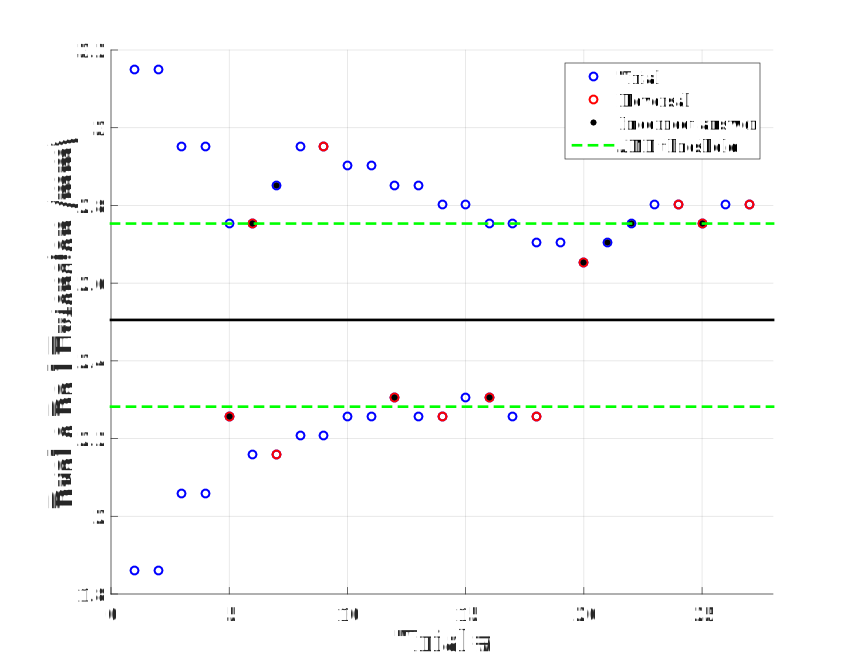
\includegraphics[scale=0.4]{fig/stairway}
  \caption{An example of the ascending and descending staircase procedure used in this experiment.}
  \label{stairway}
\end{figure}

%\newpage

\section{Apparatus and Procedure}

The apparatus consisted of the prototype, a flat PTFE surface mounted upon four load cells (Measurement Specialties FX1901), three motion capture cameras (OptiTrack Flex:V100R2) and a computer with a mouse. The load cells, amplified by Texas Instruments INA125P amplifiers, were used to measure the normal force applied to the surface and were digitized and recorded at 500~Hz by the prototype's microcontroller. The motion capture cameras, sampled at 100~Hz, tracked the position of the subject's right foot during trials. All experimental data was streamed via USB to a Unity3D\footnote{\url{https://unity3d.com/}} program, which also acted as the user interface.

Subjects were required to sit in front of the computer screen and wore the prototype on their right foot while listening to pink noise. This was done to ensure that motor actuation and ambient environment noises were not heard. The elevated PTFE surface was placed on the floor slightly in front of the subject such that their right foot could easily slide back and forth by retraction and extension of the knee. To begin a double staircase, subjects clicked a button on screen. An arrow then prompted the user to select the first stimulus, which was done by sliding their right foot back towards themselves until the prototype's heel mechanism was no longer in contact with the surface, leaving the brake pads unencumbered. A panel on screen then turned red to notify the subject not to move while the motor positioned the brake pads. Once positioned, a different panel turned green to signify that the stimulus was ready to be tested. To gauge slipperiness, the subject slid their right foot back and forth along the PTFE surface. Selecting the second stimulus involved the same process of sliding the right foot back and waiting for brake pad positioning. Subjects were required to identify the stimulus that had the greatest sliding resistance by mouse click and were permitted to toggle between the two stimuli as desired. Upon answering, the user was prompted by an arrow to activate the first stimulus of the succeeding trial. Motor actuations lasted around 500~ms, or less, and were not reported as being heard or felt by the subjects.

After each double staircase converged, the prototype sole and the PTFE surface were wiped clean of PTFE flakes to minimize their self-lubricating effects and thus improve consistency of environmental conditions. In addition, subjects were asked to complete a questionnaire based on the NASA-TLX\footnote{\url{http://humansystems.arc.nasa.gov/groups/tlx/}} to assess task difficulty. Before each subject's participation, the PTFE surface and prototype sole were sanded with 600 and 1000 grit sandpaper and subsequently cleaned with isopropyl alcohol. Figure \ref{perception_interface} illustrates the interface. Figures \ref{perception_apparatus_fiducial} and \ref{perception_slide_fiducial} show the physical layout of the experimental setup. 



\begin{figure*}[t!]
    \centering
    
    \begin{subfigure}[t]{0.5\textwidth}
        \centering
        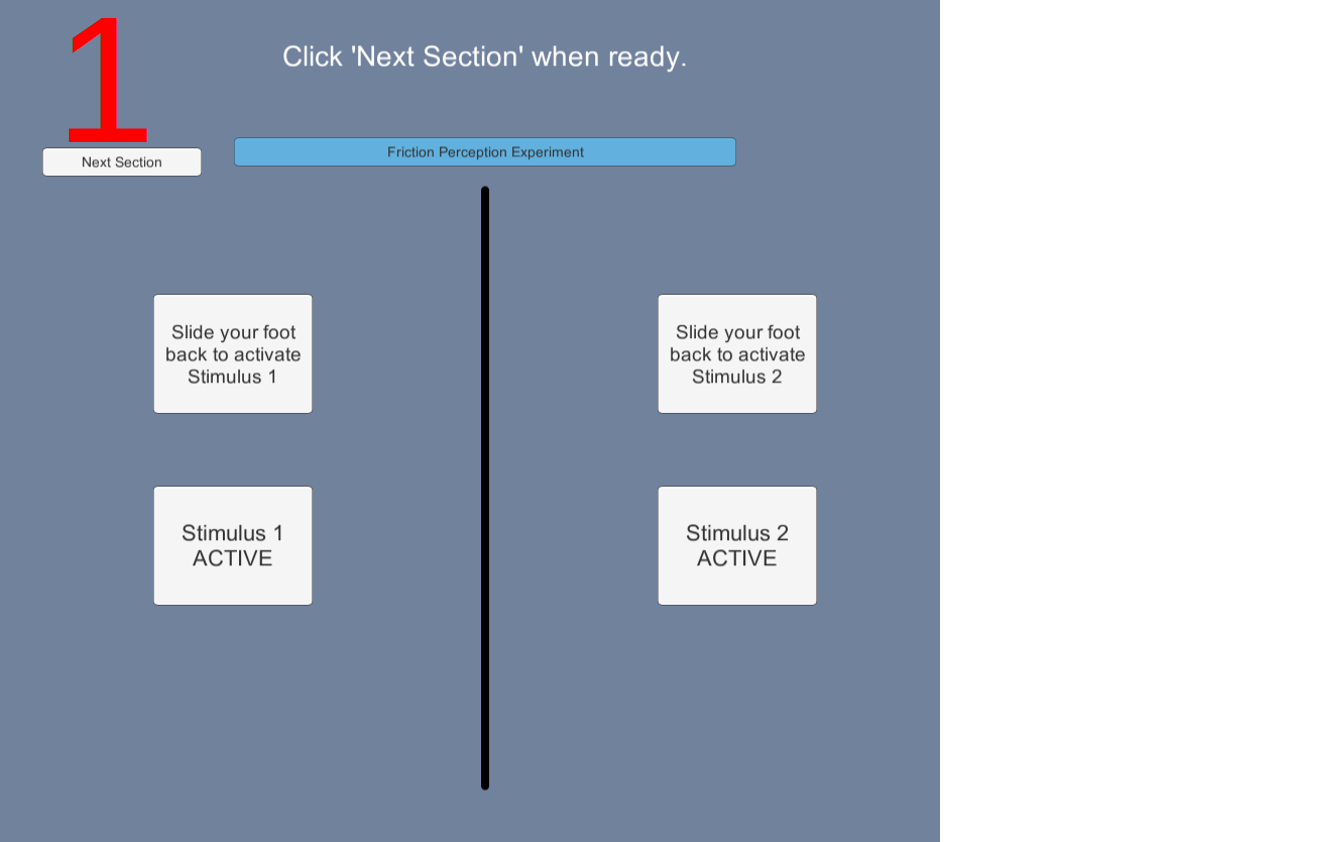
\includegraphics[scale=0.215]{fig/perception_interface1}
        \caption{User is prompted to begin the evaluation.}
    \end{subfigure}%
    ~ 
    \begin{subfigure}[t]{0.5\textwidth}
        \centering
        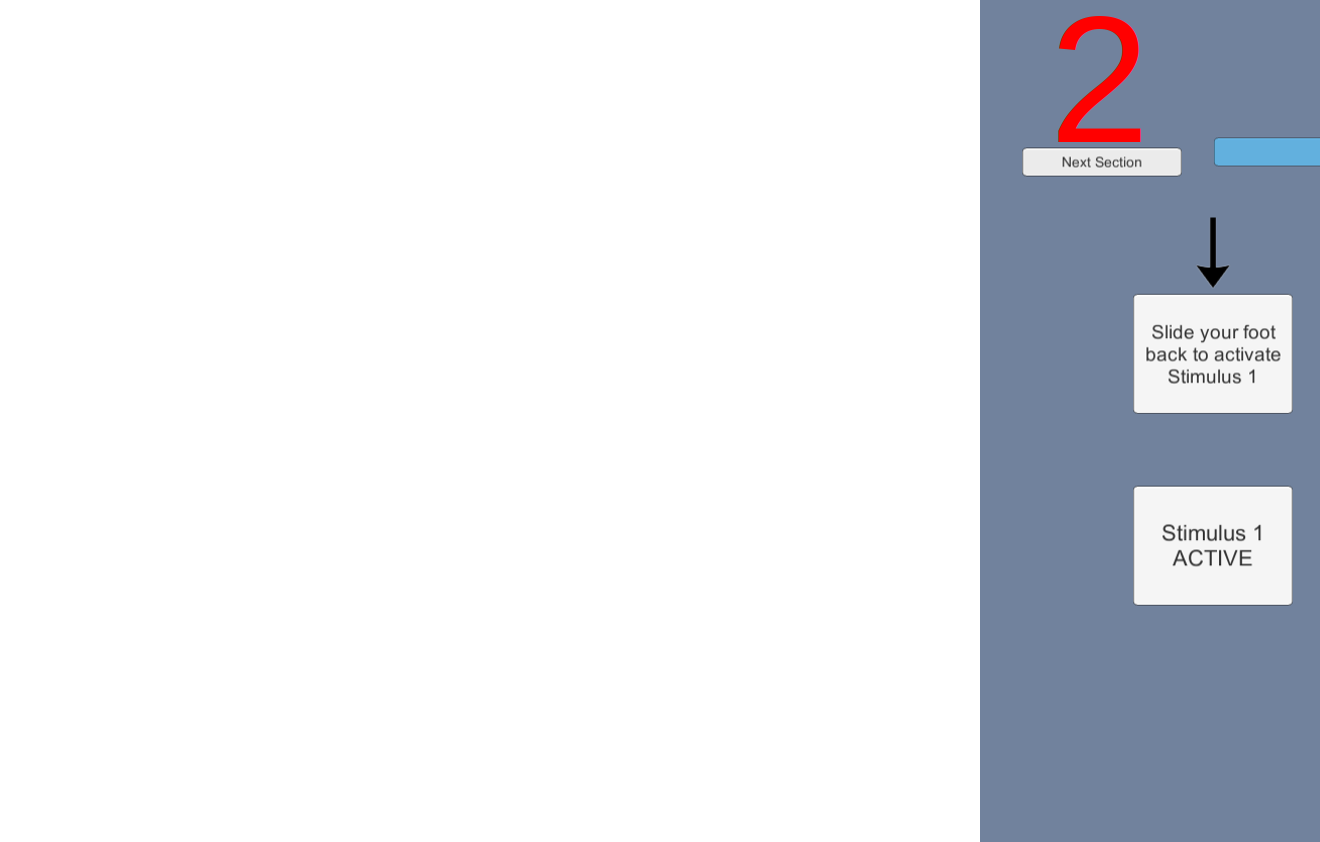
\includegraphics[scale=0.215]{fig/perception_interface2}
        \caption{Arrow directs user to activate the first stimulus.}
    \end{subfigure}
    ~
    \begin{subfigure}[t]{0.5\textwidth}
        \centering
        
\includegraphics[scale=0.215]{fig/perception_interface3}
        \caption{Panel turns red to signify actuation.}
    \end{subfigure}%
    ~ 
    \begin{subfigure}[t]{0.5\textwidth}
        \centering
        
\includegraphics[scale=0.215]{fig/perception_interface4}
        \caption{First stimulus active. Activate second stimulus when ready.}
    \end{subfigure}
    ~
    \begin{subfigure}[t]{0.5\textwidth}
        \centering
        
\includegraphics[scale=0.215]{fig/perception_interface5}
        \caption{Panel turns red to signify actuation.}
    \end{subfigure}%
    ~ 
    \begin{subfigure}[t]{0.5\textwidth}
        \centering
        
\includegraphics[scale=0.215]{fig/perception_interface6}
        \caption{Second stimulus active.}
    \end{subfigure}
    
    % Main caption
    \caption{The perception experiment user interface. Following activation of the second stimulus, the subjects either gave their evaluation or activated the first stimulus again. Following an answer, the subjects would repeat the sequence starting from the second step.}
    \label{perception_interface}
\end{figure*}

\clearpage


\begin{figure}[tpb]
  \centering
  \includegraphics[scale=0.08]{fig/perception_apparatus_fiducial}
  \caption{Experiment apparatus with annotations.}
  \label{perception_apparatus_fiducial}
\end{figure}

%\clearpage

\begin{figure}[h]
  \centering
  \includegraphics[scale=0.099]{fig/perception_slide_fiducial}
  \caption{Stimulus selection and testing positions of the foot. As seen in the left image the brake pads were unencumbered during actuation. The image on the right illustrates the motion profile used to test a stimulus.}
  \label{perception_slide_fiducial}
\end{figure} 


\section{Results}

\ilja{The results section 4.3 conflates JNDs with Weber fractions. They are, however, not the same thing. Weber fractions are JNDs scaled with respect to the reference value. While JND are expected to increase as the reference value increases, Weber fractions are typically constant (which is apparently not true for the current results) (see Gescheider, 1997, Psychophysics: The Fundamentals). At the very least the writing needs to be checked so that the conflation is eliminated; an easy solution is to report both the JNDs and the Weber fractions.}

\dan{Both JNDs and Weber fractions now included.}

%** convergence based upon final 4 reversals
%% 2710,4210,5050 ==> 1.34~mm, 2.09~mm and 2.51~mm ~(0.15, 0.225, and 0.3)
A total of eight subjects (2F~/~6M) aged 22~--~79 ($\mu=32$,~$\sigma=17.9$), voluntarily consented to participate in the study, which was approved by the McGill Research Ethics Board. Experimentation lasted 50~--~80 minutes and subjects were compensated \$10 for their time and efforts. A pre-experiment questionnaire was administered, revealing that five subjects' dominant foot was their right and that a single participant had consistent voluntary exposure to slippery surfaces due to winter sports. Despite having more experience, this subject's data was analyzed in the same manner as all other subjects.

\dan{Modified this section as warranted.} The JNDs and their Weber fractions are shown in Figures \ref{JND_normal_boxplot} and \ref{JND_weber_boxplot}. Figure \ref{tlx} displays the recorded TLX data. A Weber fraction is the expression of a JND as a percentage of its reference stimulus (i.e., if the friction discrimination perception threshold is 1~mm for a 3~mm brake pad extension reference, the JND is 33\%). This is done in accordance with Weber's law, which states that the JND between two stimuli varies proportionally with their magnitudes \cite{gescheider1997psychophysics,bau2010teslatouch} (i.e., the Weber fraction is expected to be relatively constant for each stimulus tested). In this work, the JND for each brake pad extension tested was taken as the mean JND of its two associated staircases in this work.

% temperature difference required between two surfaces while both hands are touching different surfaces.

% Traditional JND's
\begin{figure}[bhtp]
  \centering
  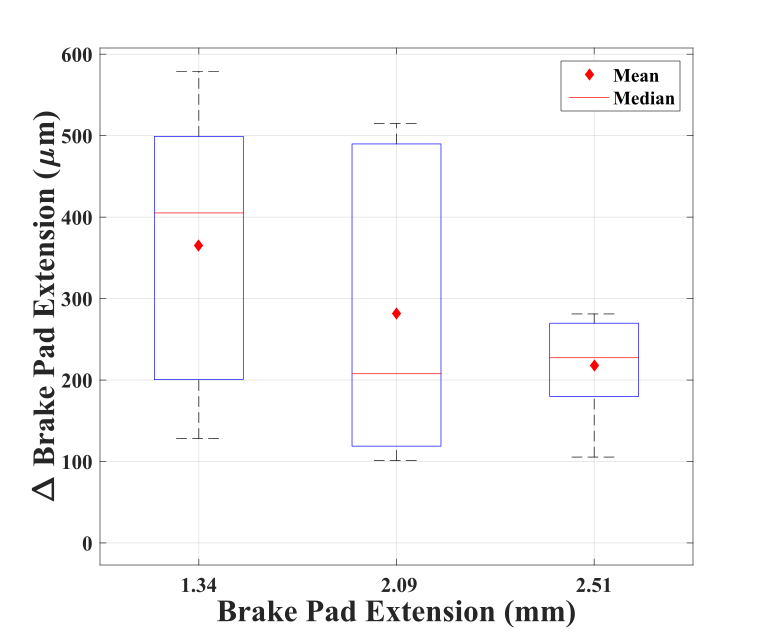
\includegraphics[scale=0.45]{fig/JND_normal_boxplot}
  \caption{Box plots of the JNDs for each of the brake pad extensions tested.%Red diamonds represent the mean values of each JND distribution, which were 0.27, 0.13 and 0.09, respectively. Red horizontal lines represent the distribution median.
  }
  \label{JND_normal_boxplot}
\end{figure}

% JND's expressed as weber fractions
\begin{figure}[bhtp]
  \centering
  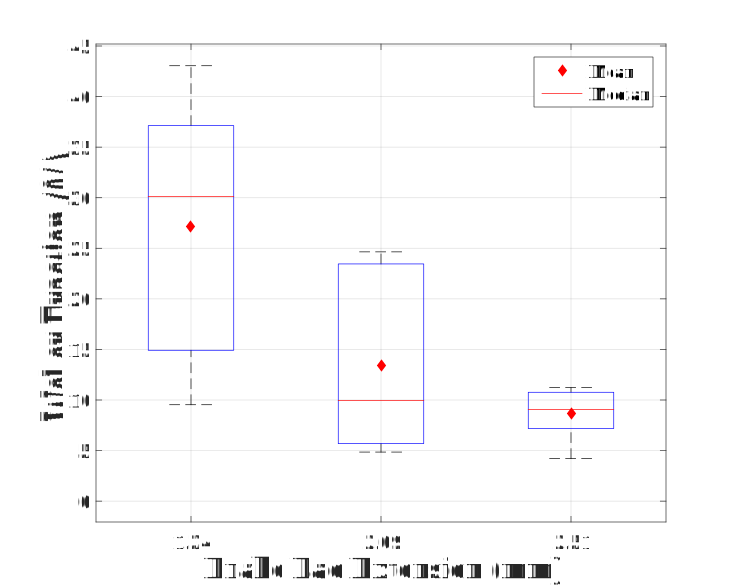
\includegraphics[scale=0.45]{fig/JND_weber_boxplot}
  \caption{Box plots of the Weber fractions for the three brake pad extensions tested.
\ilja{The label on the y-axis says the values are \%, but the actual values are proportions. I suggest changing the values to percentages, to match the discussing in the text.}
  \dan{Agreed and changed.}
  %Red diamonds represent the mean values of each JND distribution, which were 0.27, 0.13 and 0.09, respectively. Red horizontal lines represent the distribution median.
  }
  \label{JND_weber_boxplot}
\end{figure}

Performing a one-factor repeated measures ANOVA on the data reveals a significant effect on the JND of sliding friction with respect to brake pad extension ($F_{2,14}=9.14, p<0.01$). Mauchly's test confirmed that the assumption of sphericity had not been violated ($F=0.58, p=0.2$). Further inspection, focussing on the differences between each reference, reveals significant differences between the 1.34~mm and 2.51~mm extensions ($F_{1,7}=16.45, p<0.01$) and the 1.34~mm and 2.09~mm extensions ($F_{1,7}=6.05, p<0.05$). No significant difference was found between the JNDs of sliding friction for the 2.09~mm and 2.51~mm extensions ($F_{1,7}=2.67, p=0.15$).


\begin{figure}[bhtp]
  \centering
  \includegraphics[scale=0.3]{fig/tlx}
  \caption{Box plots of the TLX data recorded following the completion of each double staircase.}
  \label{tlx}
\end{figure}


\section{Discussion}

\subsection{Just-Noticeable Differences}

% Greater brake pad extensions were not tested to ensure preservation of the foam.

Weber fractions in relation to friction discrimination have been reported to fall in a range of 10~--~27\% \cite{jones2013application}. In addition, friction discrimination studies have found that the JNDs of sliding friction decrease as the COF increases \cite{provancher2009fingerpad}. While this is consistent with the findings of this experiment, we note that most friction discrimination studies seen in the literature use the pad of one's finger \cite{provancher2009fingerpad,samur2009psychophysical,bau2010teslatouch}.

As the brake pad extension was increased, (i.e., at higher coefficients of friction) a sharp decline of the mean and variance of the JNDs was seen and found to be statistically significant. Further analysis showed that the significance in the differences was only valid for the most slippery (smallest) brake pad extension in comparison to the other two extensions tested. The declining variances suggest a wider range of slip sensory resolutions for low-friction situations with respect to the subjects tested. The reduction of means suggests that from a sliding friction perception standpoint, the prototype exhibits binary behaviour. More precisely, there is a small range of brake pad extension where our ability to perceive changes in sliding friction improves its resolution as the brake pad extension increases. As such, we hypothesize that there are two friction perception levels: high-resolution for large brake pad extensions and low-resolution for small brake pad extensions, as greater increments are required for stimulus differences to be detected. We suspect that the increased pressure applied to the brake pad faces is the driving factor in this finding and there is likely a pressure threshold where the effect of the brake pads becomes dominant in regards to sliding friction perception. Based on this information, it appears that humans could consistently discern between two brake pad extensions using our prototype, perhaps three, if greater brake pad extensions are used. The reasoning for this estimation is the statistical nature of discrimination thresholds. There are no exact points above or below a stimulus where a difference is guaranteed to be detected. Responses related to stimulus detection are constantly dependent on the state of the subject and their environment.


%\jer{re-reading that several times, I'm still not sure you're conveying what is intended.  As I understand the text, you're saying that the ability of subjects to perceive changes in friction improves, the greater the extension of the brake pad, but only for a very small range of extensions.  How is this binary?  It doesn't seem consistent with what follows.} \dan{I meant that the subject's perception is binary, as in, when there is small brake pad extension we have poor perceptual resolution and when appreciable brake pad extension is present we have improved perceptual resolution. There is a small brake pad extension range over which our perceptual resolution appears to improve considerably. Given that the smallest extension's JND is significantly different from the other two, I feel it is logical to conclude that perception characteristic is somewhat binary. The following sentence has been added.}

%\jer{but isn't it the case that a large brake extension corresponds to a large change in friction coefficient?  If so, then perception of this change isn't high resolution!  Perhaps easiest to discuss in person.} \dan{In person discussion would certainly be better. It is definitely the case that a large brake pad extension implies a higher COF, but differences between 2 friction stimuli can be detected with smaller changes in brake pad extension, when taken as a percentage of total brake pad extension. My statement about high/low resolution makes the assumption that the COF and brake pad extension both increase linearly, which is relatively true when looking at Figure \ref{cof_vs_bpe}. Most simply put, larger changes in brake pad extension are required for stimulus differences to be detected for small brake pad extensions.}\jer{ok, I get it now.}


\subsection{Likert Scales}

The factors evaluated by the TLX remained relatively constant over the duration of the experiment. This, in combination with reduced distress and pace, as well as midrange scores for effort, and physical and mental demands, likely spoke to the monotony of the task, and suggests that subjects were at least moderately comfortable. Increased success levels over time may indicate a growing confidence in perception judgement as the experiment progressed. At the beginning of the experiment, subjects often reported experiencing difficulty and uncertainty in differentiating between the friction stimuli presented to them.

\subsection{Experimental Shortcomings}

While our findings are confirmed by agreement with comparable studies, the experimental method employed was non ideal. PTFE is a self-lubricating material and flakes when it is rubbed, which resulted in PTFE pieces littered about the sliding surface and coated on the brake pads after each double staircase. As such, the sliding environment was not kept in an ideally consistent condition.

The inherent monotony of the experiment was further amplified by the playing of pink noise. In addition to a long run time, these factors made subjects fatigued or disinterested and created difficulty in remaining focussed. To combat this, the total number of reversals was initially set at a relatively low value of eight. Following experimentation, it was discovered that some of the staircases were terminated early (i.e., before the prescribed number of reversals had taken place). In the current analysis, if more than six reversals are present in a staircase, the remaining reversals are not considered. While effective at reducing run time, higher numbers of reversals are generally used to obtain an accurate estimation of discrimination thresholds \cite{cornsweet1962staircase,levesque2011enhancing}.

Lastly, closed-loop control of the brake pad extension would have assisted in attempting to maintain consistent stimuli levels throughout the experiment. It would also allow brake pad actuation to occur with pressure on the prototype's heel. Thus, the interface could have been designed such that stimulus changes were done using a more time-conscious method, not requiring repositioning of the foot.


\section{Conclusion}

As seen in related research \cite{cohen1994psychophysical} and everyday life, the human foot is not an ideal friction sensor. Continued research in this area is necessary to adequately quantify our ability to perceive changes in sliding friction. This served as a secondary motivation for this study, which was primarily done to give insight as to how the prototype may be most effectively applied in sliding scenarios.

Our analysis suggests that the perception of our prototype can be discretized into two friction settings: low friction and high friction. As highlighted in Chapter \ref{design_characterization}, this could be improved by better controlling the surface area of high-friction material in contact with the floor. We found that human perceptual resolution improves considerably as the brake pads become further extended, due to increased pressure on their high-friction rubber faces. This is not a new finding and is seen elsewhere in the literature \cite{provancher2009fingerpad}, though testing is usually done with a finger pad and over a larger range of static COFs. We also note that the human perceptual resolution of sliding friction narrows its distribution as the static COF increases.
%for surface conditions with low static COFs ($\mu_s \textless 0.3$) has a wide distribution

This information is important for researchers looking to develop or use foot-based variable-friction technology as it provides insight as to the characteristics and capabilities of this friction-varying method. In a practical sense, it can be used for the design of perceptible and imperceptible friction modulation situations. A perceptible friction modulation task may include sending a tactile pattern using the prototype, where a designer would have to ensure that the brake pad extension is noticeably different to communicate meaningful signals. An imperceptible change may be necessary for a simple environment modification (e.g., changing the simulation of dry grass to wet grass). 


\chapter{Foot-Controlled Pointing using a Variable-Friction Foot Device}
\label{foot_pointing}

This chapter presents an optimized foot-controlled pointing system employing our variable friction prototype shoe. The overall objective was to characterize the system in order to evaluate its viability in replacing or augmenting conventional pointing devices.


\section{Introduction}

Foot-controlled pointing interfaces have existed almost since the inception of computers \cite{english1967display} but are often overlooked in the commercial HCI domain. This is demonstrated by a lack of prevalence in today's markets, which exhibit a narrowed focus on hand-operated peripherals. While effective, these interfaces often hamper productivity and become ineffectual in circumstances where our hands are task overloaded (e.g., machine shops, operating rooms, desktop environments). In the literature regarding foot-operated interfaces, we find that the foot is better suited to simple tasks (e.g., gestures) not requiring accuracy or fine motor control. One of the aims of this study was to apply assistive tactics that allowed the foot to become an accurate pointing tool.

Variable friction was introduced somewhat recently to HCI and has been shown to augment pointing performance, usability and user experience in hand-controlled interfaces. With respect to pointing, high-friction target regions can assist users by making targets sticky, while the remainder of the interaction space is low-friction. The result of such an addition is reduced target overshoot and simplified fine motor control when positioned in a high-friction region. Usability improves with variable friction as it adds a haptic feedback element to computing that may be more effective than traditional vibration and adds an enhanced sense of realism in using an artificial interface \cite{levesque2011enhancing}. Given superior usability and pointing, the overall user experience is ameliorated.

We employ a device capable of generating variable friction to foot-controlled pointing in this study. Designing a variable-friction pointing system, using our prototype, required special consideration due to latency of the brake pad actuation. Generating a noticeable change in the COF elicited by the shoe cannot be done instantaneously, unlike other implementations using mechanical vibration or electrovibration. In this case, the brake pads must be driven a distance necessary to ensure the effects of high-friction are experienced. Distance and velocity thresholds were used to determine the point in time at which an actuation occurred, such that target regions were guaranteed to be high-friction and the surrounding area low-friction.

\ilja{The hypothesis for the foot pointing experiment (P40) is not explicit enough (e.g., "will [...] elicit the same effects as it sees in hand-operated context". What effects?}

\dan{Further detail added: "(i.e., augmentation of pointing performance, usability and user experience)". This is mentioned earlier in the section.}

We hypothesized that applying variable friction to foot pointing will not only elicit the same effects as it sees in hand-operated contexts (i.e., augmentation of pointing performance, usability and user experience), but provide further clarity as to the potential of the human foot for use in tasks requiring precision comparable to what is expected of our hands. Our analysis focussed on objective, quantitative evaluation of pointing performance, however, subjective measures were taken as well. We chose to test two interface modes: constant low friction and variable friction. A constant high-friction interface was neglected since pilot testing gave clear indication that significantly increased effort was required and reduced TPs would result. With similar reasoning, the concept of low-friction targets and high-friction surrounding regions was not tested, though this was mainly due to the lack of a sticky target \cite{levesque2011enhancing}.

\section{Method}

To test our hypotheses and characterize the system, our attention is turned to Fitts' Law. As described in Section \ref{pointing_eval}, Fitts' Law is a predictive model for human movement time used in the evaluation of pointing devices. The implementation made use of \textit{FittsStudy},\footnote{\url{https://depts.washington.edu/aimgroup/proj/fittsstudy/}} a free application developed at the University of Washington supporting the execution and basic analysis of both 1D and 2D ISO 9241-9 tasks, which has been used in a number of publications \cite{wobbrock2008error,wobbrock2011modeling,wobbrock2011effects,velloso2015interactions}.

Subjects were required to use both friction interfaces to complete the 1D and 2D tasks for nine movement conditions. The movement conditions had amplitudes $A=\{300,600,1000\}$ and widths $W=\{20,60,128\}$, which gave an index of difficulty range $I\!D=\{1.74-5.67\}$. Each movement condition had a total of fifteen trials, the first four of which were discarded to mask learning effects, resulting in 396 recorded movements per subject.

%Set of ID's: (1.7415,2.5078,2.585,3.1396,3.4594,4,4.143,4.9542,5.6724)

To ensure suppression of the bias of learning effects, a number of measures were taken. The presentation of each combination of interface and dimensionality was based on a Latin squares design. The order of movement conditions within each task was randomized by the software. Before each evaluation began, the subjects completed three trials for each combination of interface, task dimensionality and movement condition. Subjects were required to listen to pink noise in addition to wearing sound suppressing earmuffs during all phases of the evaluation in order to mask the motor's loud actuation.


\section{Apparatus and Procedure}

The apparatus consisted of the prototype, a slanted PTFE surface, three motion capture cameras (OptiTrack Flex:V100R2), a 24-inch  1920~$\times$~1080 LCD monitor and an ASUS TP500LN laptop computer (Intel\textregistered~Core\texttrademark~i7-4510U CPU $@$ 2~GHz, 8~GB RAM, Windows 10) with a mouse. The motion capture cameras, sampled at 100~Hz, tracked the position of the subject's right foot during the evaluation, which was streamed via USB to a modified version of \textit{FittsStudy} as cursor position input. %The modified software analyzed this input and communicated with the prototypes microcontroller for brake pad extension control.

Subjects wore the prototype on their right foot, which they slid on the slanted PTFE surface to control the mouse cursor. The position of the foot on the PTFE surface was mapped in direct proportion to the screen (i.e., absolute positioning). To begin a movement condition, subjects clicked on a light blue highlighted shape, which was a rectangle in the 1D case and a circle in the 2D case. Figure \ref{1D_2D} depicts the two task layouts. Upon clicking, the shape would instantly fade to a faint gray colour and another shape at a different location would highlight light blue to indicate itself as the succeeding cursor target. This process repeated until the fifteen trials had been completed, at which time the subject was required to press a key to begin the following movement condition. Subjects used a conventional mouse left-click to indicate a selection since our interests were specifically focussed on the human ability to control cursor position. Rather than forcing subjects to learn a new selection modality, we opted to simplify this aspect of the task with the intent of minimizing dwell time. Subjects were instructed to move the cursor to the succeeding target as quickly and accurately as possible, with emphasis on speed. The pace of the experiment was described to subjects as being comparable to a work environment.

Before each subject's participation, the PTFE surface and prototype sole were sanded with 600 and 1000 grit sandpaper and subsequently cleaned with isopropyl alcohol. Following the practice set of trials and each combination of interface and dimensionality, the prototype sole and the PTFE surface were wiped clean of PTFE flakes. Figure \ref{pointing_apparatus} shows the physical layout of the experimental setup.

Upon conclusion of the experiment, subjects were required to complete a questionnaire quantifying their levels of comfort, effort and fatigue. The questionnaire enquired on a number of aspects related to the interface such as perception of variable friction, subject's preferences (e.g., 1D versus 2D), user's suggested improvements, strategies employed and difficulties encountered.

\begin{figure}%[tpb]
  \centering
  \includegraphics[scale=0.08]{fig/pointing_apparatus}
  \caption{Apparatus used in the foot-controlled pointing Fitts' characterization. The PTFE surface was set on an incline to facilitate a greater range of motion when sliding the foot whilst sitting.}
  \label{pointing_apparatus}
\end{figure}

%Interface figures, (if necessary)
%\begin{figure}[tpb]
%  \centering
%  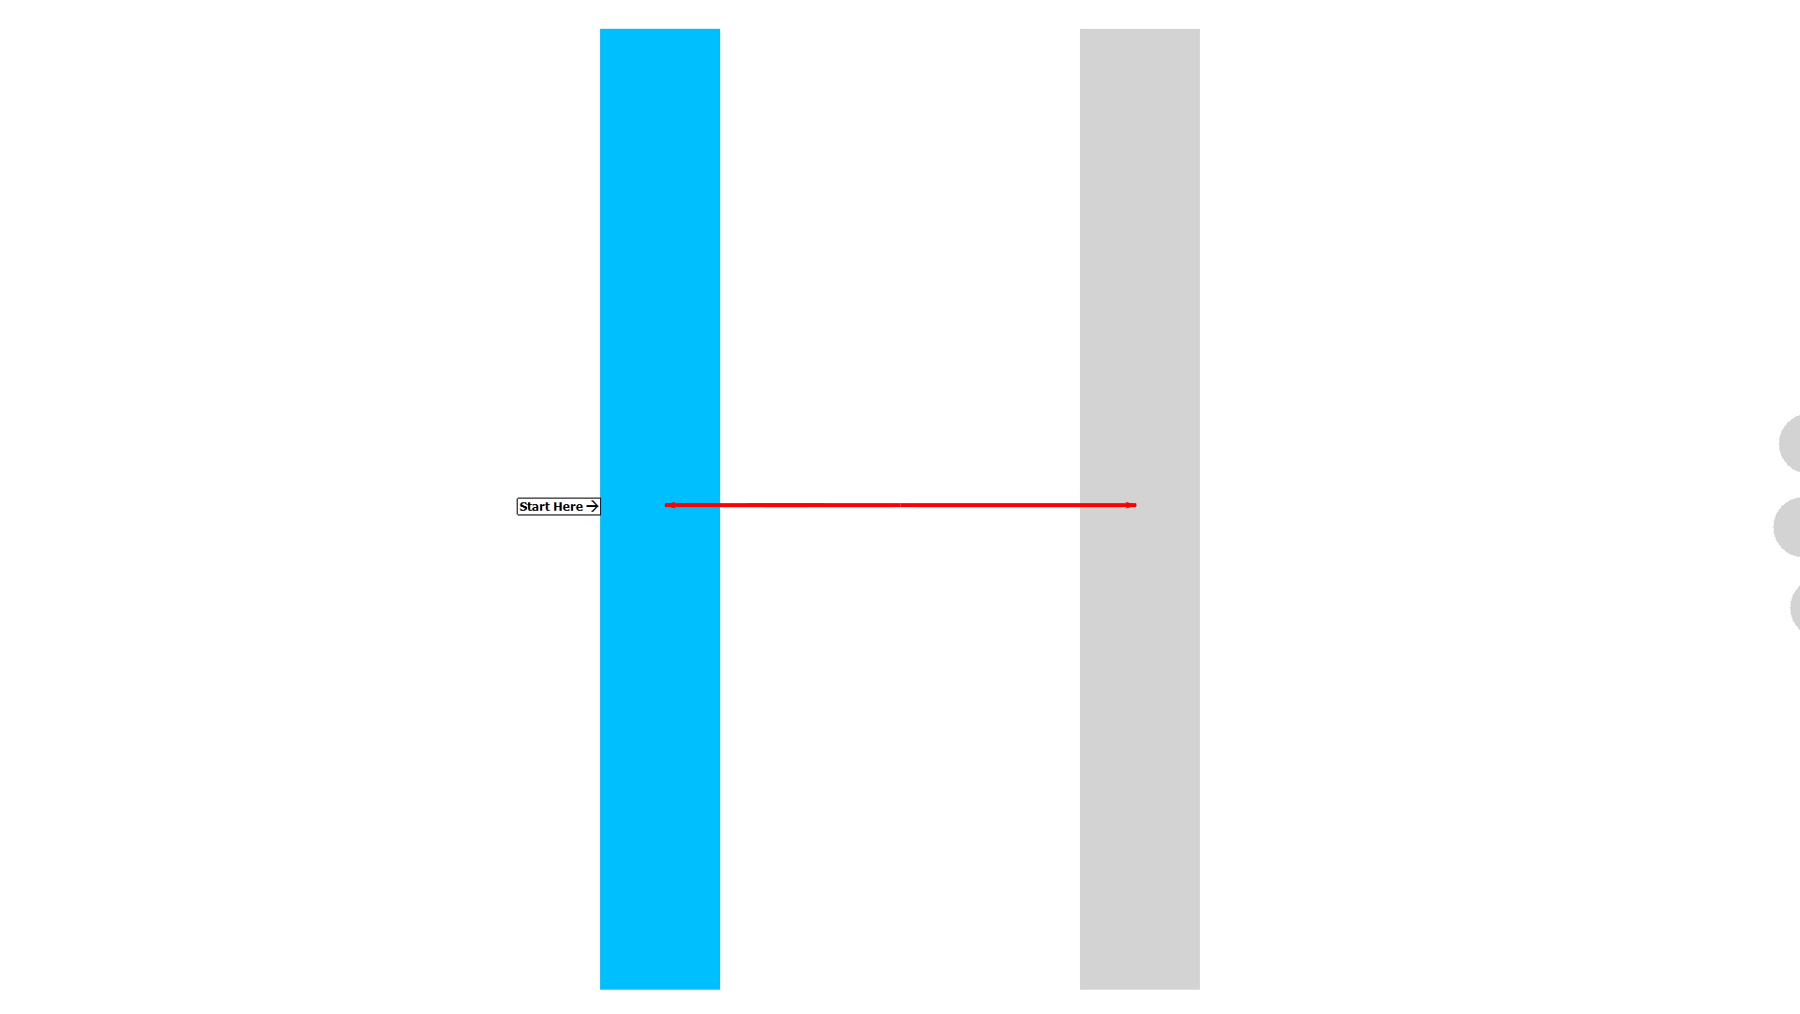
\includegraphics[scale=0.2]{fig/1D_2D}
%  \caption{On the left, the original 1D Fitts' task is seen. On the right the 2D ISO 9241-9 task layout is seen.}
%  \label{1D_2D}
%\end{figure}

\section{Results}

A total of twelve subjects (6F~/~6M) aged 20~--~33 ($\mu=24.3$,~$\sigma=3.8$), voluntarily consented to participate in the study, which was first approved by the McGill Research Ethics Board. Experimentation lasted 40~--~50 minutes and subjects were compensated \$10 for their time and efforts. A pre-experiment questionnaire was administered, revealing that eleven of the subjects were right-foot dominant, while the other was ambidextrous. Three of the subjects rarely encountered foot-operated interfaces (e.g., car driving, piano/organ playing), but the remaining nine dealt with them on a consistent basis (i.e., more than twice per week). Please note, an additional subject was ran but was excluded from the analysis due to failure to follow experiment instructions.

Table \ref{fitts_TP_table} summarizes the Fitts' models and their associated coefficients of determination as well as the mean TPs and percentage errors for each combination of interface and dimensionality. Figure~\ref{fitts_models} shows graphical illustration of the movement models for each combination of interface and dimensionality.




A two-factor repeated measures ANOVA was used to analyze the TP data, revealing significant effects of both friction interface ($F_{1,11}=21.31, p<0.001$) and task dimensionality ($F_{1,11}=350.40, p<0.001$). No interaction was found between these two factors ($F_{1,11}=0.53, p=0.48$). Application of Mauchly's test confirmed that the assumption of sphericity had not been violated ($F=0.72, p=0.68$). Further inspection, comparing the TPs of constant and variable friction with respect to task dimensionality reveal significant differences between the interfaces for the 1D ($F_{1,11}=10.87, p<0.01$) and 2D tasks ($F_{1,11}=5.07, p<0.05$). Graphical illustration of the TPs can be seen in Figure \ref{CF_VF_boxplot}.

Post-experiment questionnaire data reveal clear opinions as to the general perception of the interface and how an effective, more user-friendly iteration of the design could be developed. The distribution of responses to Likert scale questions can be seen in Figure \ref{likert_boxplot}.

\begin{table}[pb]
\centering
\caption{Fitts' Law movement time models, their coefficients of determination and associated TPs and error rates.}
\label{fitts_TP_table}
\begin{tabular}{@{}l|ll|ll@{}}
\toprule
\textbf{Interface} & \textbf{Movement Model} & \textbf{R$^2$} & \textbf{TP (bits/s)} & \textbf{\% Error} \\ \midrule
1D CF              & $MT=I\!D\times341-7$         & 0.74                         & 3.04                 & 6.38              \\
1D VF              & $MT=I\!D\times271-156$       & 0.74                         & 3.22                 & 6.40               \\
2D CF              & $MT=I\!D\times619-363$       & 0.76                         & 2.09                 & 10.93             \\
2D VF              & $MT=I\!D\times470-22$        & 0.80                         & 2.21                 & 8.19              \\ \bottomrule
\end{tabular}
\end{table}

\begin{figure}[htpb]
  \centering
  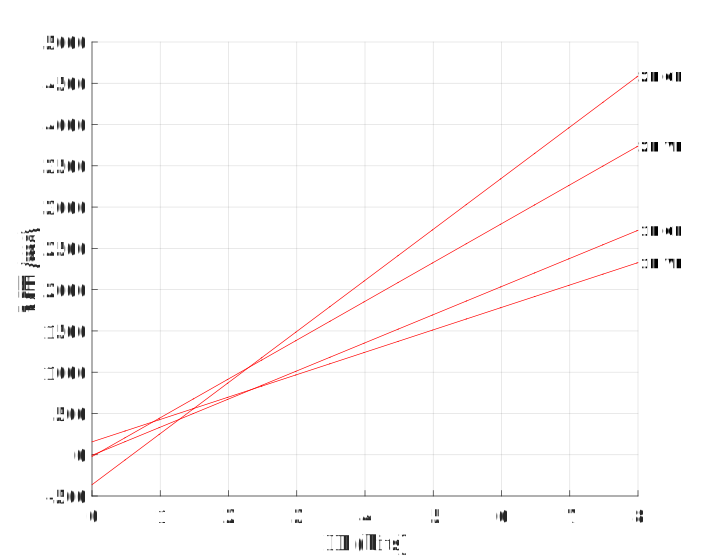
\includegraphics[scale=0.45]{fig/fitts_models}
  \caption{Graphical illustration of the Fitts' Law movement models for each condition tested.%Distribution means are represented by a red diamond, while medians are represented by a horizontal red line. Outliers are represented as red crosses.
  }
  \label{fitts_models}
\end{figure}


\begin{figure}[tpb]
  \centering
  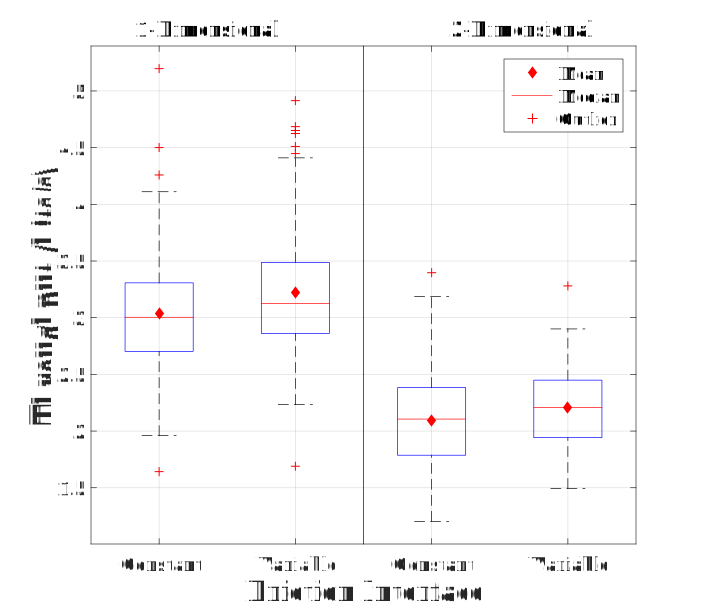
\includegraphics[scale=0.45]{fig/CF_VF_boxplot}
  \caption{Box plots of all four combinations of friction interface and task dimensionality.%Distribution means are represented by a red diamond, while medians are represented by a horizontal red line. Outliers are represented as red crosses.
  }
  \label{CF_VF_boxplot}
\end{figure}

\newpage %separate the figures...

\begin{figure}[tpb]
  \centering
  \includegraphics[scale=0.55]{fig/likert_boxplot}
  \caption{Box plots of the Likert scale data collected in the post-experiment questionnaire.%Distribution means are represented by a red diamond, while medians are represented by a blue circle filled in white, having a black point at the centre. Outliers are represented as blue circles filled in white.
  }
  \label{likert_boxplot}
\end{figure}


\section{Discussion}

% footnote 13, towards a standard for pointing devices

\subsection{Movement Models}

\ilja{Reference is made to "relatively gradual slopes" (P44) but they are not shown.}

\dan{The slopes are seen in the table, but they can now also be seen graphically as well. The graph was added in the previous section following the table.}

In regards to the 1D cases, relatively gradual slopes are seen along with intercepts falling in the acceptable range of -200~--~400 ms \cite{soukoreff2004towards} (see Figure~\ref{fitts_models}). The slopes indicate that subjects experienced a gradual decrease in performance as the ID increases, which is expected given the simplicity of the 1D task. The slopes of the 2D models highlight that an additional dimension nearly doubles the movement time required to point for tasks with the same ID. We note that longer movement times are especially prevalent for small target widths. A clear peculiarity seen in the 2D CF case is its low intercept. This is attributed to the inherent difficulty of accurate 2D foot-pointing on a slippery surface. While reduced friction minimizes the effort required to move the foot, a lack of accurate fine motor control is observed. Subjects had the tendency to overshoot targets by a small distance and subsequently attempt correction only to overshoot again. Thus, considerable time was spent attempting correction. The same characteristic is not seen in the 1D CF case, most likely due to heel rotation. As we will discuss later, subjects used heel rotation extensively in the 1D task, as it was a highly effective, natural movement. We also note that curved trajectories were often seen in both 1D and 2D tasks.


\begin{figure}[tpb]
  \centering
  \includegraphics[scale=0.35]{fig/overshoot_2D_CF}
  \caption{An example of recurring overshoot seen in the 2D CF task.}
  \label{overshoot_2D_CF}
\end{figure}

\subsection{Throughputs}

Performance in each combination of interface and task dimensionality was greater than expected. Although this is, to our knowledge, only the second foot-controlled pointing system analyzed using ISO 9241-9 \cite{velloso2015interactions}, a clear difference in performance is seen by comparison with the other analysis. The 1D case exhibits TPs greater than the maxima recorded for trackballs, touchpads and joysticks, as shown in Table \ref{ISO_comparison}. While such a comparison is clearly biased, it quantifies the high degree of performance the foot has for simple tasks. With respect to the 2D cases, more typical TPs are observed in comparison to conventional pointing systems. At this point, it would be unrealistic to consider the system as an effective competitor to the mouse.

We attribute our system's performance primarily to the inclined low-friction surface. Minimal effort in sliding in combination with sticky targets greatly simplifies foot-controlled pointing. Observed error rates are comparable to conventional pointing devices, though our 2D cases are somewhat high. We hypothesize that with practice, improved TPs and reduced error rates would be seen and establish the system as a clear competitor with touchpads and trackballs. Referring back to the original objective of the experiment, an evaluation should be applied to pointing devices such that cursor control and keyboard manipulation are simultaneously required. For example, a task where large blocks of text must be repositioned and new text must be composed. This would truly exemplify a need for foot-controlled interfaces.

\subsection{Post-Experiment Data}

\subsubsection{Likert Scales}

The Likert scale assessment reflects quite positively on the system. With regards to ease of use, comfort and smoothness we note a clear indication of user appreciation for the interface, owing again mainly to the low-friction surface and perhaps the use of familiar mouse clicks as a selection modality. The midrange values of physical effort scores can be explained by an extended experiment time and lack of experience with the body kinematics associated with foot pointing. We attribute the mental effort scores to the inherent required concentration when performing Fitts' tasks. Lastly, we point out that low fatigue scores are observed following a minimum of thirty minutes of continuous pointing activity. Such results are likely helpful for the adoption of new peripherals.  

\subsubsection{Perceptions, Preferences, Strategies and Challenges}

%on a number of interface specifics concerning perceptions, preferences, strategies and challenges, which we will now briefly discuss.

% Perception/prefence
Seven of the subjects reported perceiving the friction modulation, five of whom felt vibration in addition to increased sliding resistance. Only two of these subjects actually preferred the variable-friction interface. Those who disliked variable friction complained of feeling a lack of control and difficulty in manipulation as desired. Given the improved results of the variable friction modality, we hypothesize that subjects merely perceived a lack of control, due to the increased sliding resistance, rather than having actually experienced one. Four subjects preferred the 2D task for its challenge, while the remainder enjoyed the simplicity of a single dimension. The most preferred direction of movement was diagonal, along the \textit{northwest}/\textit{southeast} axis, where north is located at the toe and south is located at the heel.  We presume this preference is credited to a physiological predisposition, as similar findings are seen in other publications \cite{alexander2012putting}.

% Challenges/strategies
Fine motor control, especially when applied to small-target pointing, was reported as the most challenging aspect of the experiment. Two specific strategies were noted: firm placement of the left foot for superior control and heel rotation for improved accuracy. Only two of the subjects cited firm foot placement, but all utilized heel rotation. Subjects generally employed heel rotation in low amplitude 1D tasks because of the ease of this movement and, given a single dimension, the vertical aspect of the arcing motion of the cursor could be neglected.

% Improvements (Some users suggested changing the system entirely to what could be described as a swivelling gas pedal.)
Subject's recommendations and improvements to the system were widely varied. Mainly, physical improvements were suggested as summarized below. A number of subjects noted that they could imagine the prototype as a peripheral in gaming contexts.

\begin{itemize}
	\item Subjects wanted the ability to configure the device's friction levels to their own preference. This would negate the feeling of lacking control and give users the ability to fine tune the device to their own characteristics. As such, practical implementations may include a calibration option in the design.

	\item Adding vibration feedback was suggested by a number of subjects. Given the inconsistency in sliding friction perception, we hypothesize that this feedback may cause users to overcompensate and perhaps undershoot their targets, though empirical testing is the only way to answer this question.
	
	\item Modification of the position system from an absolute one to a rate-based implementation (i.e., first-order control) may be assistive in low-amplitude movements due to the smaller displacements for reduced speeds.
	
\end{itemize}


\subsection{Experimental Shortcomings and Future Work}

In an effort to improve consistency with other pointing device analyses, our experiment made use of \textit{FittsStudy} and followed the guidelines for analysis of a pointing device as prescribed by Soukoreff and MacKenzie \cite{soukoreff2004towards}. Nonetheless, there are evident shortcomings.  In typical fashion, a wider range of IDs and a greater number of trials could have been run to better characterize system and improve confidence in the analysis. The number of trials and ID range were selected for reasons of pragmatism and time efficiency but cover appreciable ranges of amplitude, width and ID. Vibration from the motor should have been damped such that it was not perceived at all. It is possible that this vibration feedback played a role in the improved performance seen with the variable-friction interface as it may have acted as an additional feedback mechanism for target approach, perhaps indicating an ideal deceleration point \cite{akamatsu1995comparison}.

Distracting targets (i.e., targets occluding pointing trajectories) and the effects of practice require further investigation, as described in other literature \cite{levesque2011enhancing,velloso2015feet}. Positive results found when investigating the effects of distracting targets validate the application of variable friction to real interfaces. Unfortunately, designing a user interface having a pointer that does not encounter occluded target trajectories may oversimplify the interface. Validating that variable-friction interfaces remain effective with distracting targets (e.g., running a Fitts' experiment with distracters) serves as convincing evidence in regards to their usefulness.  The effects of practice have already been documented for the feet showing that improvement continues over time without an obvious plateau. Given the high degree of performance with our system, we believe that practice could make it a serious competitor to conventional pointing devices.

Our method of implementation, from a software perspective, for the variable-friction interface was effective but is not currently scalable due to empirical classification. That is, the distance and velocity thresholds of brake pad actuation were based on pilot testing and not computed dynamically, meaning that it was possible for actuation to be late or early. Predictive methods, such as Kalman filters, could be employed to improve accuracy and scalability of the system in terms of determining the distance and velocity thresholds at which actuation occurs.


\section{Conclusion}

A variable-friction foot-controlled pointing system was presented and analyzed under the ISO 9241-9 standard for pointing device evaluation. The effects of variable friction were found to improve pointing performance by a statistically significant margin in both 1D and 2D tasks. Constrained, low-friction surfaces are comfortable, easy to manipulate and generate little fatigue when constantly used over extended periods of time. Applying this concept to hand-operated peripherals and evaluating performance serves as a potential direction of further pointing research. A number of necessary minor adjustments became apparent following the analysis of the post-experiment questionnaire data. These include further addition of haptic feedback, modifying the positioning method and focus on specific gestures (i.e., heel rotation) in future iterations.

We found further evidence that the foot may compete with traditional hand-operated pointing devices. The notion that the foot is better suited to coarse grained, non-accurate tasks is supported by evidence from this experiment, but this analysis indicates that with assistive techniques our feet can be useful in tasks requiring precision. This finding may be important for other researchers investigating foot-operated interfaces.

Evaluation of foot-controlled pointing systems against other pointing devices should be performed with tasks requiring simultaneous cursor control and keyboard manipulation to demonstrate the improved efficiency foot pointing may offer. In addition, the effects of practice require further exploration \cite{velloso2015feet}. These two factors represent the next steps this research effort should take.


\chapter{Conclusion}

%\section{Conclusion}

The development and application of a foot-worn variable-friction prototype was carried out. The original motivations of the study came from a need to create on-demand slip situations for use in balance training, rehabilitation and virtual reality. Properly focussing the scope of the work, in addition to ensuring the longevity of the prefabricated variable-friction mechanism, conveniently narrowed the design space to low force contexts. To ensure this, human experimentation was done with the subjects in a sitting position.

Given the narrowed scope, a flat-soled prototype was fabricated and characterized in terms of its static COF for ranges of both brake pad extension and mass that we expected the prototype to encounter. An approximate static COF range of 0.11~--~0.4 was found, meaning that surfaces ranging in slipperiness from ice to wet asphalt could be simulated.

Human perception of sliding friction while using the prototype was then evaluated. Three brake pad extensions, equally spaced in relation to their static COFs, were evaluted for their JNDs using an adaptive staircase procedure. The JNDs of the prototype quickly decreased as the COF (i.e., brake pad extension) increased, resulting in a JND range of 9~--~27\%. The JND of the lowest friction setting was found to be significantly different from the other two JNDs, implying that human perceptual resolution of sliding friction increased with further brake pad extension. We attribute this finding to increased pressure on the high-friction faces of the brake pads. Based on this evaluation, we hypothesize that the prototype could be discretized into two or three perceptually distinct friction settings.

The prototype was then applied in the field of foot-controlled pointing. Evaluation was performed using ISO 9241-9 in 1D and 2D tasks. Two interface modes were tested: constant low friction and variable friction. The variable-friction interface was designed such that target regions were high friction and the remainder of the interaction space was low friction. Reasonable performance was seen in the evaluation, placing the system in the same tier as touchpads and trackballs. Based on performance results of the constant-low-friction tasks, we can conclude that the use of low friction was a driving factor in performance. The variable-friction mode saw the best performance and was found to be significantly different from its constant-friction counterpart. The results suggest that the foot can perform well in tasks requiring nontrivial accuracy when assistive methods are applied appropriately.



%\section{Future Work}
%
%To establish foot-controlled pointing as a clear improver of efficiency, the system should be analyzed against

%========== End Chapters


%========== Bibliography
\typeout{}
\begin{singlespace}
  \bibliography{thesisHorodniczy}
  \bibliographystyle{ieeetr}
\end{singlespace}

\end{document}
